\documentclass[10pt,journal,compsoc]{IEEEtran}
% *** CITATION PACKAGES ***
%
% \ifCLASSOPTIONcompsoc
%   % IEEE Computer Society needs nocompress option
%   % requires cite.sty v4.0 or later (November 2003)
%   \usepackage[nocompress]{cite}
% \else
%   % normal IEEE
%   \usepackage{cite}
% \fi
\usepackage[numbers,square,sort,comma]{StyFiles/natbib}
\usepackage{StyFiles/natbibspacing}

% External Document
% \usepackage{xr}
% \externaldocument{nips_2021_appendix}

%% Contents
\usepackage{makeidx}

%% Figures
\usepackage[pdftex]{graphicx}
\DeclareGraphicsExtensions{.pdf,.jpeg,.png}
\usepackage{hyperref}
\usepackage{xcolor}         % colors
\usepackage{subcaption}

%% Features
\usepackage[utf8]{inputenc} % allow utf-8 input
\usepackage[T1]{fontenc}    % use 8-bit T1 fonts
\usepackage{StyFiles/fancyhdr}
\usepackage{StyFiles/wrapfig}
\usepackage{url}
\usepackage{makecell}
\usepackage{textcomp}
\usepackage{booktabs}
\usepackage{multirow}
\usepackage[normalem]{ulem}
\useunder{\uline}{\ul}{}

%% Formats
\usepackage{nicefrac}       % compact symbols for 1/2, etc.
\usepackage{microtype}      % microtypography
% \usepackage[toc,page]{appendix}
% \usepackage[font=small,labelfont=bf]{caption}
% \usepackage[font=footnotesize]{subfig}
\usepackage{StyFiles/hyphenat}
% correct bad hyphenation here
\hyphenation{op-tical net-works semi-conduc-tor}

%% Algos
\usepackage{StyFiles/algorithm}
\usepackage{StyFiles/algorithmic}
% Todo: remove algorithm2e?
\usepackage[algo2e,ruled,vlined,linesnumbered]{algorithm2e}
% Do NOT use the algorithm floating environment provided by
% algorithm.sty (by the same authors) or algorithm2e.sty (by
% Christophe Fiorio) as the IEEE does not use dedicated algorithm
% float types and packages that provide these will not provide
% correct IEEE style captions.
\newcommand{\fix}{\marginpar{FIX}}
\newcommand{\new}{\marginpar{NEW}}


%% For maths
\usepackage[cmex10]{amsmath}
% Note that the amsmath package sets \interdisplaylinepenalty to 10000
% thus preventing page breaks from occurring within multiline equations. Use:
%\interdisplaylinepenalty=2500
\usepackage{amsfonts}       % blackboard math symbols
\usepackage{amssymb,amsthm}
\usepackage{array}
%%%%% NEW MATH DEFINITIONS %%%%%

\usepackage{amsmath,amsfonts,bm}

% Mark sections of captions for referring to divisions of figures
\newcommand{\figleft}{{\em (Left)}}
\newcommand{\figcenter}{{\em (Center)}}
\newcommand{\figright}{{\em (Right)}}
\newcommand{\figtop}{{\em (Top)}}
\newcommand{\figbottom}{{\em (Bottom)}}
\newcommand{\captiona}{{\em (a)}}
\newcommand{\captionb}{{\em (b)}}
\newcommand{\captionc}{{\em (c)}}
\newcommand{\captiond}{{\em (d)}}

% Highlight a newly defined term
\newcommand{\newterm}[1]{{\bf #1}}


% Figure reference, lower-case.
\def\figref#1{figure~\ref{#1}}
% Figure reference, capital. For start of sentence
\def\Figref#1{Figure~\ref{#1}}
\def\twofigref#1#2{figures \ref{#1} and \ref{#2}}
\def\quadfigref#1#2#3#4{figures \ref{#1}, \ref{#2}, \ref{#3} and \ref{#4}}
% Section reference, lower-case.
\def\secref#1{section~\ref{#1}}
% Section reference, capital.
\def\Secref#1{Section~\ref{#1}}
% Reference to two sections.
\def\twosecrefs#1#2{sections \ref{#1} and \ref{#2}}
% Reference to three sections.
\def\secrefs#1#2#3{sections \ref{#1}, \ref{#2} and \ref{#3}}
% Reference to an equation, lower-case.
\def\eqref#1{equation~\ref{#1}}
% Reference to an equation, upper case
\def\Eqref#1{Equation~\ref{#1}}
% A raw reference to an equation---avoid using if possible
\def\plaineqref#1{\ref{#1}}
% Reference to a chapter, lower-case.
\def\chapref#1{chapter~\ref{#1}}
% Reference to an equation, upper case.
\def\Chapref#1{Chapter~\ref{#1}}
% Reference to a range of chapters
\def\rangechapref#1#2{chapters\ref{#1}--\ref{#2}}
% Reference to an algorithm, lower-case.
\def\algref#1{algorithm~\ref{#1}}
% Reference to an algorithm, upper case.
\def\Algref#1{Algorithm~\ref{#1}}
\def\twoalgref#1#2{algorithms \ref{#1} and \ref{#2}}
\def\Twoalgref#1#2{Algorithms \ref{#1} and \ref{#2}}
% Reference to a part, lower case
\def\partref#1{part~\ref{#1}}
% Reference to a part, upper case
\def\Partref#1{Part~\ref{#1}}
\def\twopartref#1#2{parts \ref{#1} and \ref{#2}}

\def\ceil#1{\lceil #1 \rceil}
\def\floor#1{\lfloor #1 \rfloor}
\def\1{\bm{1}}
\newcommand{\train}{\mathcal{D}}
\newcommand{\valid}{\mathcal{D_{\mathrm{valid}}}}
\newcommand{\test}{\mathcal{D_{\mathrm{test}}}}

\def\eps{{\epsilon}}


% Random variables
\def\reta{{\textnormal{$\eta$}}}
\def\ra{{\textnormal{a}}}
\def\rb{{\textnormal{b}}}
\def\rc{{\textnormal{c}}}
\def\rd{{\textnormal{d}}}
\def\re{{\textnormal{e}}}
\def\rf{{\textnormal{f}}}
\def\rg{{\textnormal{g}}}
\def\rh{{\textnormal{h}}}
\def\ri{{\textnormal{i}}}
\def\rj{{\textnormal{j}}}
\def\rk{{\textnormal{k}}}
\def\rl{{\textnormal{l}}}
% rm is already a command, just don't name any random variables m
\def\rn{{\textnormal{n}}}
\def\ro{{\textnormal{o}}}
\def\rp{{\textnormal{p}}}
\def\rq{{\textnormal{q}}}
\def\rr{{\textnormal{r}}}
\def\rs{{\textnormal{s}}}
\def\rt{{\textnormal{t}}}
\def\ru{{\textnormal{u}}}
\def\rv{{\textnormal{v}}}
\def\rw{{\textnormal{w}}}
\def\rx{{\textnormal{x}}}
\def\ry{{\textnormal{y}}}
\def\rz{{\textnormal{z}}}

% Random vectors
\def\rvepsilon{{\mathbf{\epsilon}}}
\def\rvtheta{{\mathbf{\theta}}}
\def\rva{{\mathbf{a}}}
\def\rvb{{\mathbf{b}}}
\def\rvc{{\mathbf{c}}}
\def\rvd{{\mathbf{d}}}
\def\rve{{\mathbf{e}}}
\def\rvf{{\mathbf{f}}}
\def\rvg{{\mathbf{g}}}
\def\rvh{{\mathbf{h}}}
\def\rvu{{\mathbf{i}}}
\def\rvj{{\mathbf{j}}}
\def\rvk{{\mathbf{k}}}
\def\rvl{{\mathbf{l}}}
\def\rvm{{\mathbf{m}}}
\def\rvn{{\mathbf{n}}}
\def\rvo{{\mathbf{o}}}
\def\rvp{{\mathbf{p}}}
\def\rvq{{\mathbf{q}}}
\def\rvr{{\mathbf{r}}}
\def\rvs{{\mathbf{s}}}
\def\rvt{{\mathbf{t}}}
\def\rvu{{\mathbf{u}}}
\def\rvv{{\mathbf{v}}}
\def\rvw{{\mathbf{w}}}
\def\rvx{{\mathbf{x}}}
\def\rvy{{\mathbf{y}}}
\def\rvz{{\mathbf{z}}}

% Elements of random vectors
\def\erva{{\textnormal{a}}}
\def\ervb{{\textnormal{b}}}
\def\ervc{{\textnormal{c}}}
\def\ervd{{\textnormal{d}}}
\def\erve{{\textnormal{e}}}
\def\ervf{{\textnormal{f}}}
\def\ervg{{\textnormal{g}}}
\def\ervh{{\textnormal{h}}}
\def\ervi{{\textnormal{i}}}
\def\ervj{{\textnormal{j}}}
\def\ervk{{\textnormal{k}}}
\def\ervl{{\textnormal{l}}}
\def\ervm{{\textnormal{m}}}
\def\ervn{{\textnormal{n}}}
\def\ervo{{\textnormal{o}}}
\def\ervp{{\textnormal{p}}}
\def\ervq{{\textnormal{q}}}
\def\ervr{{\textnormal{r}}}
\def\ervs{{\textnormal{s}}}
\def\ervt{{\textnormal{t}}}
\def\ervu{{\textnormal{u}}}
\def\ervv{{\textnormal{v}}}
\def\ervw{{\textnormal{w}}}
\def\ervx{{\textnormal{x}}}
\def\ervy{{\textnormal{y}}}
\def\ervz{{\textnormal{z}}}

% Random matrices
\def\rmA{{\mathbf{A}}}
\def\rmB{{\mathbf{B}}}
\def\rmC{{\mathbf{C}}}
\def\rmD{{\mathbf{D}}}
\def\rmE{{\mathbf{E}}}
\def\rmF{{\mathbf{F}}}
\def\rmG{{\mathbf{G}}}
\def\rmH{{\mathbf{H}}}
\def\rmI{{\mathbf{I}}}
\def\rmJ{{\mathbf{J}}}
\def\rmK{{\mathbf{K}}}
\def\rmL{{\mathbf{L}}}
\def\rmM{{\mathbf{M}}}
\def\rmN{{\mathbf{N}}}
\def\rmO{{\mathbf{O}}}
\def\rmP{{\mathbf{P}}}
\def\rmQ{{\mathbf{Q}}}
\def\rmR{{\mathbf{R}}}
\def\rmS{{\mathbf{S}}}
\def\rmT{{\mathbf{T}}}
\def\rmU{{\mathbf{U}}}
\def\rmV{{\mathbf{V}}}
\def\rmW{{\mathbf{W}}}
\def\rmX{{\mathbf{X}}}
\def\rmY{{\mathbf{Y}}}
\def\rmZ{{\mathbf{Z}}}

% Elements of random matrices
\def\ermA{{\textnormal{A}}}
\def\ermB{{\textnormal{B}}}
\def\ermC{{\textnormal{C}}}
\def\ermD{{\textnormal{D}}}
\def\ermE{{\textnormal{E}}}
\def\ermF{{\textnormal{F}}}
\def\ermG{{\textnormal{G}}}
\def\ermH{{\textnormal{H}}}
\def\ermI{{\textnormal{I}}}
\def\ermJ{{\textnormal{J}}}
\def\ermK{{\textnormal{K}}}
\def\ermL{{\textnormal{L}}}
\def\ermM{{\textnormal{M}}}
\def\ermN{{\textnormal{N}}}
\def\ermO{{\textnormal{O}}}
\def\ermP{{\textnormal{P}}}
\def\ermQ{{\textnormal{Q}}}
\def\ermR{{\textnormal{R}}}
\def\ermS{{\textnormal{S}}}
\def\ermT{{\textnormal{T}}}
\def\ermU{{\textnormal{U}}}
\def\ermV{{\textnormal{V}}}
\def\ermW{{\textnormal{W}}}
\def\ermX{{\textnormal{X}}}
\def\ermY{{\textnormal{Y}}}
\def\ermZ{{\textnormal{Z}}}

% Vectors
\def\vzero{{\bm{0}}}
\def\vone{{\bm{1}}}
\def\vmu{{\bm{\mu}}}
\def\vtheta{{\bm{\theta}}}
\def\va{{\bm{a}}}
\def\vb{{\bm{b}}}
\def\vc{{\bm{c}}}
\def\vd{{\bm{d}}}
\def\ve{{\bm{e}}}
\def\vf{{\bm{f}}}
\def\vg{{\bm{g}}}
\def\vh{{\bm{h}}}
\def\vi{{\bm{i}}}
\def\vj{{\bm{j}}}
\def\vk{{\bm{k}}}
\def\vl{{\bm{l}}}
\def\vm{{\bm{m}}}
\def\vn{{\bm{n}}}
\def\vo{{\bm{o}}}
\def\vp{{\bm{p}}}
\def\vq{{\bm{q}}}
\def\vr{{\bm{r}}}
\def\vs{{\bm{s}}}
\def\vt{{\bm{t}}}
\def\vu{{\bm{u}}}
\def\vv{{\bm{v}}}
\def\vw{{\bm{w}}}
\def\vx{{\bm{x}}}
\def\vy{{\bm{y}}}
\def\vz{{\bm{z}}}

% Elements of vectors
\def\evalpha{{\alpha}}
\def\evbeta{{\beta}}
\def\evepsilon{{\epsilon}}
\def\evlambda{{\lambda}}
\def\evomega{{\omega}}
\def\evmu{{\mu}}
\def\evpsi{{\psi}}
\def\evsigma{{\sigma}}
\def\evtheta{{\theta}}
\def\eva{{a}}
\def\evb{{b}}
\def\evc{{c}}
\def\evd{{d}}
\def\eve{{e}}
\def\evf{{f}}
\def\evg{{g}}
\def\evh{{h}}
\def\evi{{i}}
\def\evj{{j}}
\def\evk{{k}}
\def\evl{{l}}
\def\evm{{m}}
\def\evn{{n}}
\def\evo{{o}}
\def\evp{{p}}
\def\evq{{q}}
\def\evr{{r}}
\def\evs{{s}}
\def\evt{{t}}
\def\evu{{u}}
\def\evv{{v}}
\def\evw{{w}}
\def\evx{{x}}
\def\evy{{y}}
\def\evz{{z}}

% Matrix
\def\mA{{\bm{A}}}
\def\mB{{\bm{B}}}
\def\mC{{\bm{C}}}
\def\mD{{\bm{D}}}
\def\mE{{\bm{E}}}
\def\mF{{\bm{F}}}
\def\mG{{\bm{G}}}
\def\mH{{\bm{H}}}
\def\mI{{\bm{I}}}
\def\mJ{{\bm{J}}}
\def\mK{{\bm{K}}}
\def\mL{{\bm{L}}}
\def\mM{{\bm{M}}}
\def\mN{{\bm{N}}}
\def\mO{{\bm{O}}}
\def\mP{{\bm{P}}}
\def\mQ{{\bm{Q}}}
\def\mR{{\bm{R}}}
\def\mS{{\bm{S}}}
\def\mT{{\bm{T}}}
\def\mU{{\bm{U}}}
\def\mV{{\bm{V}}}
\def\mW{{\bm{W}}}
\def\mX{{\bm{X}}}
\def\mY{{\bm{Y}}}
\def\mZ{{\bm{Z}}}
\def\mBeta{{\bm{\beta}}}
\def\mPhi{{\bm{\Phi}}}
\def\mLambda{{\bm{\Lambda}}}
\def\mSigma{{\bm{\Sigma}}}

% Tensor
\DeclareMathAlphabet{\mathsfit}{\encodingdefault}{\sfdefault}{m}{sl}
\SetMathAlphabet{\mathsfit}{bold}{\encodingdefault}{\sfdefault}{bx}{n}
\newcommand{\tens}[1]{\bm{\mathsfit{#1}}}
\def\tA{{\tens{A}}}
\def\tB{{\tens{B}}}
\def\tC{{\tens{C}}}
\def\tD{{\tens{D}}}
\def\tE{{\tens{E}}}
\def\tF{{\tens{F}}}
\def\tG{{\tens{G}}}
\def\tH{{\tens{H}}}
\def\tI{{\tens{I}}}
\def\tJ{{\tens{J}}}
\def\tK{{\tens{K}}}
\def\tL{{\tens{L}}}
\def\tM{{\tens{M}}}
\def\tN{{\tens{N}}}
\def\tO{{\tens{O}}}
\def\tP{{\tens{P}}}
\def\tQ{{\tens{Q}}}
\def\tR{{\tens{R}}}
\def\tS{{\tens{S}}}
\def\tT{{\tens{T}}}
\def\tU{{\tens{U}}}
\def\tV{{\tens{V}}}
\def\tW{{\tens{W}}}
\def\tX{{\tens{X}}}
\def\tY{{\tens{Y}}}
\def\tZ{{\tens{Z}}}


% Graph
\def\gA{{\mathcal{A}}}
\def\gB{{\mathcal{B}}}
\def\gC{{\mathcal{C}}}
\def\gD{{\mathcal{D}}}
\def\gE{{\mathcal{E}}}
\def\gF{{\mathcal{F}}}
\def\gG{{\mathcal{G}}}
\def\gH{{\mathcal{H}}}
\def\gI{{\mathcal{I}}}
\def\gJ{{\mathcal{J}}}
\def\gK{{\mathcal{K}}}
\def\gL{{\mathcal{L}}}
\def\gM{{\mathcal{M}}}
\def\gN{{\mathcal{N}}}
\def\gO{{\mathcal{O}}}
\def\gP{{\mathcal{P}}}
\def\gQ{{\mathcal{Q}}}
\def\gR{{\mathcal{R}}}
\def\gS{{\mathcal{S}}}
\def\gT{{\mathcal{T}}}
\def\gU{{\mathcal{U}}}
\def\gV{{\mathcal{V}}}
\def\gW{{\mathcal{W}}}
\def\gX{{\mathcal{X}}}
\def\gY{{\mathcal{Y}}}
\def\gZ{{\mathcal{Z}}}

% Sets
\def\sA{{\mathbb{A}}}
\def\sB{{\mathbb{B}}}
\def\sC{{\mathbb{C}}}
\def\sD{{\mathbb{D}}}
% Don't use a set called E, because this would be the same as our symbol
% for expectation.
\def\sF{{\mathbb{F}}}
\def\sG{{\mathbb{G}}}
\def\sH{{\mathbb{H}}}
\def\sI{{\mathbb{I}}}
\def\sJ{{\mathbb{J}}}
\def\sK{{\mathbb{K}}}
\def\sL{{\mathbb{L}}}
\def\sM{{\mathbb{M}}}
\def\sN{{\mathbb{N}}}
\def\sO{{\mathbb{O}}}
\def\sP{{\mathbb{P}}}
\def\sQ{{\mathbb{Q}}}
\def\sR{{\mathbb{R}}}
\def\sS{{\mathbb{S}}}
\def\sT{{\mathbb{T}}}
\def\sU{{\mathbb{U}}}
\def\sV{{\mathbb{V}}}
\def\sW{{\mathbb{W}}}
\def\sX{{\mathbb{X}}}
\def\sY{{\mathbb{Y}}}
\def\sZ{{\mathbb{Z}}}

% Entries of a matrix
\def\emLambda{{\Lambda}}
\def\emA{{A}}
\def\emB{{B}}
\def\emC{{C}}
\def\emD{{D}}
\def\emE{{E}}
\def\emF{{F}}
\def\emG{{G}}
\def\emH{{H}}
\def\emI{{I}}
\def\emJ{{J}}
\def\emK{{K}}
\def\emL{{L}}
\def\emM{{M}}
\def\emN{{N}}
\def\emO{{O}}
\def\emP{{P}}
\def\emQ{{Q}}
\def\emR{{R}}
\def\emS{{S}}
\def\emT{{T}}
\def\emU{{U}}
\def\emV{{V}}
\def\emW{{W}}
\def\emX{{X}}
\def\emY{{Y}}
\def\emZ{{Z}}
\def\emSigma{{\Sigma}}

% entries of a tensor
% Same font as tensor, without \bm wrapper
\newcommand{\etens}[1]{\mathsfit{#1}}
\def\etLambda{{\etens{\Lambda}}}
\def\etA{{\etens{A}}}
\def\etB{{\etens{B}}}
\def\etC{{\etens{C}}}
\def\etD{{\etens{D}}}
\def\etE{{\etens{E}}}
\def\etF{{\etens{F}}}
\def\etG{{\etens{G}}}
\def\etH{{\etens{H}}}
\def\etI{{\etens{I}}}
\def\etJ{{\etens{J}}}
\def\etK{{\etens{K}}}
\def\etL{{\etens{L}}}
\def\etM{{\etens{M}}}
\def\etN{{\etens{N}}}
\def\etO{{\etens{O}}}
\def\etP{{\etens{P}}}
\def\etQ{{\etens{Q}}}
\def\etR{{\etens{R}}}
\def\etS{{\etens{S}}}
\def\etT{{\etens{T}}}
\def\etU{{\etens{U}}}
\def\etV{{\etens{V}}}
\def\etW{{\etens{W}}}
\def\etX{{\etens{X}}}
\def\etY{{\etens{Y}}}
\def\etZ{{\etens{Z}}}

% The true underlying data generating distribution
\newcommand{\pdata}{p_{\rm{data}}}
% The empirical distribution defined by the training set
\newcommand{\ptrain}{\hat{p}_{\rm{data}}}
\newcommand{\Ptrain}{\hat{P}_{\rm{data}}}
% The model distribution
\newcommand{\pmodel}{p_{\rm{model}}}
\newcommand{\Pmodel}{P_{\rm{model}}}
\newcommand{\ptildemodel}{\tilde{p}_{\rm{model}}}
% Stochastic autoencoder distributions
\newcommand{\pencode}{p_{\rm{encoder}}}
\newcommand{\pdecode}{p_{\rm{decoder}}}
\newcommand{\precons}{p_{\rm{reconstruct}}}

\newcommand{\laplace}{\mathrm{Laplace}} % Laplace distribution

\newcommand{\E}{\mathbb{E}}
\newcommand{\Ls}{\mathcal{L}}
\newcommand{\R}{\mathbb{R}}
\newcommand{\emp}{\tilde{p}}
\newcommand{\lr}{\alpha}
\newcommand{\reg}{\lambda}
\newcommand{\rect}{\mathrm{rectifier}}
\newcommand{\softmax}{\mathrm{softmax}}
\newcommand{\sigmoid}{\sigma}
\newcommand{\softplus}{\zeta}
\newcommand{\KL}{D_{\mathrm{KL}}}
\newcommand{\Var}{\mathrm{Var}}
\newcommand{\standarderror}{\mathrm{SE}}
\newcommand{\Cov}{\mathrm{Cov}}
% Wolfram Mathworld says $L^2$ is for function spaces and $\ell^2$ is for vectors
% But then they seem to use $L^2$ for vectors throughout the site, and so does
% wikipedia.
\newcommand{\normlzero}{L^0}
\newcommand{\normlone}{L^1}
\newcommand{\normltwo}{L^2}
\newcommand{\normlp}{L^p}
\newcommand{\normmax}{L^\infty}

\newcommand{\parents}{Pa} % See usage in notation.tex. Chosen to match Daphne's book.

\DeclareMathOperator*{\argmax}{arg\,max}
\DeclareMathOperator*{\argmin}{arg\,min}

\DeclareMathOperator{\sign}{sign}
\DeclareMathOperator{\Tr}{Tr}
\let\ab\allowbreak


%% Commands
\newcommand{\red}[1]{\textcolor[HTML]{EB4335}{#1}}
\newcommand{\blue}[1]{\textcolor[HTML]{4285F4}{#1}}
\newcommand{\linkblue}[1]{\textcolor[HTML]{2E649E}{#1}}

\definecolor{myLinkColor}{rgb}{0.18,0.39,0.62}
\hypersetup{
  colorlinks=true,
  linkcolor=myLinkColor,
  filecolor=myLinkColor,
  urlcolor=myLinkColor,
  citecolor=myLinkColor,
}

% Math
\newcommand{\mmqp}[3]{\textrm{\sc MaxMarginQP}\!\left(\{\by_t, #1\}_{t=1}^{T}, #2, #3\right)}
\newcommand{\energy}[1]{\ensuremath{E\!\left(#1\right)}}
\newcommand{\bigCI}{\mathrel{\text{\scalebox{1.07}{$\perp\mkern-10mu\perp$}}}}
% Indicator Function
\newcommand{\ind}[1]{\ensuremath{\makebox[.3ex][l]{[}\makebox{[}#1\makebox[.3ex][l]{]}\makebox{]}}}

% Reference Shortcuts
\renewcommand{\citename}{\citet}
\renewcommand{\cite}{\citep}
\newcommand{\appref}[1]{Appendix~\ref{#1}}

% Text
\newcommand{\eg}{e.g.,~}
\newcommand{\ie}{i.e.,~}


%% Environments
\newtheorem{thm}{Theorem}[section]
\newtheorem{cor}[thm]{Corollary}
\newtheorem{lem}[thm]{Lemma}
\newtheorem{prop}[thm]{Proposition}
\newtheorem{obs}[thm]{Observation}
\newtheorem{defn}[thm]{Definition}

% *** SUBFIGURE PACKAGES ***
%\ifCLASSOPTIONcompsoc
%  \usepackage[caption=false,font=footnotesize,labelfont=sf,textfont=sf]{subfig}
%\else
%  \usepackage[caption=false,font=footnotesize]{subfig}
%\fi
% subfig.sty, written by Steven Douglas Cochran, is the modern replacement
% for subfigure.sty, the latter of which is no longer maintained and is
% incompatible with some LaTeX packages including fixltx2e. However,
% subfig.sty requires and automatically loads Axel Sommerfeldt's caption.sty
% which will override IEEEtran.cls' handling of captions and this will result
% in non-IEEE style figure/table captions. To prevent this problem, be sure
% and invoke subfig.sty's "caption=false" package option (available since
% subfig.sty version 1.3, 2005/06/28) as this is will preserve IEEEtran.cls
% handling of captions.
% Note that the Computer Society format requires a sans serif font rather
% than the serif font used in traditional IEEE formatting and thus the need
% to invoke different subfig.sty package options depending on whether
% compsoc mode has been enabled.
%
% The latest version and documentation of subfig.sty can be obtained at:
% http://www.ctan.org/pkg/subfig

% *** FLOAT PACKAGES ***
%
%\usepackage{fixltx2e}
% fixltx2e, the successor to the earlier fix2col.sty, was written by
% Frank Mittelbach and David Carlisle. This package corrects a few problems
% in the LaTeX2e kernel, the most notable of which is that in current
% LaTeX2e releases, the ordering of single and double column floats is not
% guaranteed to be preserved. Thus, an unpatched LaTeX2e can allow a
% single column figure to be placed prior to an earlier double column
% figure.
% Be aware that LaTeX2e kernels dated 2015 and later have fixltx2e.sty's
% corrections already built into the system in which case a warning will
% be issued if an attempt is made to load fixltx2e.sty as it is no longer
% needed.
% The latest version and documentation can be found at:
% http://www.ctan.org/pkg/fixltx2e

%\usepackage{stfloats}
% stfloats.sty was written by Sigitas Tolusis. This package gives LaTeX2e
% the ability to do double column floats at the bottom of the page as well
% as the top. (e.g., "\begin{figure*}[!b]" is not normally possible in
% LaTeX2e). It also provides a command:
%\fnbelowfloat
% to enable the placement of footnotes below bottom floats (the standard
% LaTeX2e kernel puts them above bottom floats). This is an invasive package
% which rewrites many portions of the LaTeX2e float routines. It may not work
% with other packages that modify the LaTeX2e float routines. The latest
% version and documentation can be obtained at:
% http://www.ctan.org/pkg/stfloats
% Do not use the stfloats baselinefloat ability as the IEEE does not allow
% \baselineskip to stretch. Authors submitting work to the IEEE should note
% that the IEEE rarely uses double column equations and that authors should try
% to avoid such use. Do not be tempted to use the cuted.sty or midfloat.sty
% packages (also by Sigitas Tolusis) as the IEEE does not format its papers in
% such ways.
% Do not attempt to use stfloats with fixltx2e as they are incompatible.
% Instead, use Morten Hogholm'a dblfloatfix which combines the features
% of both fixltx2e and stfloats:
%
% \usepackage{dblfloatfix}
% The latest version can be found at:
% http://www.ctan.org/pkg/dblfloatfix

%\ifCLASSOPTIONcaptionsoff
%  \usepackage[nomarkers]{endfloat}
% \let\MYoriglatexcaption\caption
% \renewcommand{\caption}[2][\relax]{\MYoriglatexcaption[#2]{#2}}
%\fi
% endfloat.sty was written by James Darrell McCauley, Jeff Goldberg and 
% Axel Sommerfeldt. This package may be useful when used in conjunction with 
% IEEEtran.cls'  captionsoff option. Some IEEE journals/societies require that
% submissions have lists of figures/tables at the end of the paper and that
% figures/tables without any captions are placed on a page by themselves at
% the end of the document. If needed, the draftcls IEEEtran class option or
% \CLASSINPUTbaselinestretch interface can be used to increase the line
% spacing as well. Be sure and use the nomarkers option of endfloat to
% prevent endfloat from "marking" where the figures would have been placed
% in the text. The two hack lines of code above are a slight modification of
% that suggested by in the endfloat docs (section 8.4.1) to ensure that
% the full captions always appear in the list of figures/tables - even if
% the user used the short optional argument of \caption[]{}.
% IEEE papers do not typically make use of \caption[]'s optional argument,
% so this should not be an issue. A similar trick can be used to disable
% captions of packages such as subfig.sty that lack options to turn off
% the subcaptions:
% For subfig.sty:
% \let\MYorigsubfloat\subfloat
% \renewcommand{\subfloat}[2][\relax]{\MYorigsubfloat[]{#2}}
% However, the above trick will not work if both optional arguments of
% the \subfloat command are used. Furthermore, there needs to be a
% description of each subfigure *somewhere* and endfloat does not add
% subfigure captions to its list of figures. Thus, the best approach is to
% avoid the use of subfigure captions (many IEEE journals avoid them anyway)
% and instead reference/explain all the subfigures within the main caption.
% The latest version of endfloat.sty and its documentation can obtained at:
% http://www.ctan.org/pkg/endfloat
%
% The IEEEtran \ifCLASSOPTIONcaptionsoff conditional can also be used
% later in the document, say, to conditionally put the References on a 
% page by themselves.

\begin{document}
\title{Option2Vec: Learning Temporal-State Abstraction Embeddings
  on the MDP}
%
%
% author names and IEEE memberships
% note positions of commas and nonbreaking spaces ( ~ ) LaTeX will not break
% a structure at a ~ so this keeps an author's name from being broken across
% two lines.
% use \thanks{} to gain access to the first footnote area
% a separate \thanks must be used for each paragraph as LaTeX2e's \thanks
% was not built to handle multiple paragraphs
%
%
%\IEEEcompsocitemizethanks is a special \thanks that produces the bulleted
% lists the Computer Society journals use for "first footnote" author
% affiliations. Use \IEEEcompsocthanksitem which works much like \item
% for each affiliation group. When not in compsoc mode,
% \IEEEcompsocitemizethanks becomes like \thanks and
% \IEEEcompsocthanksitem becomes a line break with idention. This
% facilitates dual compilation, although admittedly the differences in the
% desired content of \author between the different types of papers makes a
% one-size-fits-all approach a daunting prospect. For instance, compsoc 
% journal papers have the author affiliations above the "Manuscript
% received ..."  text while in non-compsoc journals this is reversed. Sigh.

\author{Chang~Li,
        Dongjin~Song,
        and~Dacheng~Tao,~\IEEEmembership{Fellow,~IEEE}% <-this % stops a space
\IEEEcompsocitemizethanks{\IEEEcompsocthanksitem Chang Li and
  Dacheng Tao were
  with the UBTECH Sydney AI Centre,
  School of Computer Science, University of Sydney,
  Sydney, NSW 2000, Australia.
  E-mail: \texttt{chli4934@uni.sydney.edu.au} 
  \texttt{dacheng.tao@sydney.edu.au}
% note need leading \protect in front of \\ to get a newline within \thanks as
% \\ is fragile and will error, could use \hfil\break instead.
\IEEEcompsocthanksitem Dongjin Song University.}% <-this % stops an unwanted space
\thanks{Manuscript received December 19, 2021}}

% note the % following the last \IEEEmembership and also \thanks - 
% these prevent an unwanted space from occurring between the last author name
% and the end of the author line. i.e., if you had this:
% 
% \author{....lastname \thanks{...} \thanks{...} }
%                     ^------------^------------^----Do not want these spaces!
%
% a space would be appended to the last name and could cause every name on that
% line to be shifted left slightly. This is one of those "LaTeX things". For
% instance, "\textbf{A} \textbf{B}" will typeset as "A B" not "AB". To get
% "AB" then you have to do: "\textbf{A}\textbf{B}"
% \thanks is no different in this regard, so shield the last } of each \thanks
% that ends a line with a % and do not let a space in before the next \thanks.
% Spaces after \IEEEmembership other than the last one are OK (and needed) as
% you are supposed to have spaces between the names. For what it is worth,
% this is a minor point as most people would not even notice if the said evil
% space somehow managed to creep in.

% The only time the second header will appear is for the odd numbered pages
% after the title page when using the twoside option.
% 
% *** Note that you probably will NOT want to include the author's ***
% *** name in the headers of peer review papers.                   ***
% You can use \ifCLASSOPTIONpeerreview for conditional compilation here if
% you desire.


% The paper headers
\markboth{Journal of \LaTeX\ Class Files,~Vol.~14, No.~8, August~2015}%
{Shell \MakeLowercase{\textit{et al.}}: Bare Demo of IEEEtran.cls for Computer Society Journals}

% The publisher's ID mark at the bottom of the page is less important with
% Computer Society journal papers as those publications place the marks
% outside of the main text columns and, therefore, unlike regular IEEE
% journals, the available text space is not reduced by their presence.
% If you want to put a publisher's ID mark on the page you can do it like
% this:
%\IEEEpubid{0000--0000/00\$00.00~\copyright~2015 IEEE}
% or like this to get the Computer Society new two part style.
%\IEEEpubid{\makebox[\columnwidth]{\hfill 0000--0000/00/\$00.00~\copyright~2015 IEEE}%
%\hspace{\columnsep}\makebox[\columnwidth]{Published by the IEEE Computer Society\hfill}}
% Remember, if you use this you must call \IEEEpubidadjcol in the second
% column for its text to clear the IEEEpubid mark (Computer Society jorunal
% papers don't need this extra clearance.)

% use for special paper notices
%\IEEEspecialpapernotice{(Invited Paper)}

% for Computer Society papers, we must declare the abstract and index terms
% PRIOR to the title within the \IEEEtitleabstractindextext IEEEtran
% command as these need to go into the title area created by \maketitle.
% As a general rule, do not put math, special symbols or citations
% in the abstract or keywords.
\IEEEtitleabstractindextext{%
\begin{abstract}
  The option framework develops options on a sample inefficient
  Semi-Markov Decision Process (SMDP) and represents each option
  computational expensively as two distributions and one
  initiation set. In this paper, we present the option-induced
  SMDP as a simple Hidden-Markov-Model-style Probabilistic
  Graphical Model (PGM), which enables representing each option
  as efficient as one embedding vector (hidden variable). We
  consider temporal and state abstraction jointly. In particular,
  we formulate the option framework as a
  Hidden-Markov-Model-style Probabilistic Graphical Model (PGM),
  thus enabling each option to be parameterized as a compact
  embedding vector. To optimize this PGM, we first propose a
  novel \emph{Markovian Option-Value function}, and prove it is
  an unbiased estimation of the conventional value function. We
  then derive a two-stage policy gradient theorem based on the
  above value function. Finally, we implement this PGM upon the
  Transformer architecture to encode options into fixed-length
  embeddings, named Option2Vec. Extensive experiments on
  challenging \textit{Mujoco} environments demonstrate
  Option2Vec's efficiency and effectiveness: under widely used
  configuration, with merely 15.8\% parameters, Option2Vec
  achieves competitive, if not better, performance compared to
  the state-of-the-art baselines on all finite horizon and
  transfer learning environments. Moreover, Option2Vec
  significantly outperforms all baselines on infinite horizon
  environments while exhibiting smaller variance, faster
  convergence, and interpretability.
\end{abstract}

% Note that keywords are not normally used for peerreview papers.
\begin{IEEEkeywords}
  The Option Framework, Hierarchical Reinforcement Learning,
  Markov Decision Process
\end{IEEEkeywords}}


% make the title area
\maketitle


% To allow for easy dual compilation without having to reenter the
% abstract/keywords data, the \IEEEtitleabstractindextext text will
% not be used in maketitle, but will appear (i.e., to be "transported")
% here as \IEEEdisplaynontitleabstractindextext when the compsoc 
% or transmag modes are not selected <OR> if conference mode is selected 
% - because all conference papers position the abstract like regular
% papers do.
\IEEEdisplaynontitleabstractindextext
% \IEEEdisplaynontitleabstractindextext has no effect when using
% compsoc or transmag under a non-conference mode.



% For peer review papers, you can put extra information on the cover
% page as needed:
% \ifCLASSOPTIONpeerreview
% \begin{center} \bfseries EDICS Category: 3-BBND \end{center}
% \fi
%
% For peerreview papers, this IEEEtran command inserts a page break and
% creates the second title. It will be ignored for other modes.
\IEEEpeerreviewmaketitle



\IEEEraisesectionheading{\section{Introduction}\label{sec:introduction}}
% Computer Society journal (but not conference!) papers do something unusual
% with the very first section heading (almost always called "Introduction").
% They place it ABOVE the main text! IEEEtran.cls does not automatically do
% this for you, but you can achieve this effect with the provided
% \IEEEraisesectionheading{} command. Note the need to keep any \label that
% is to refer to the section immediately after \section in the above as
% \IEEEraisesectionheading puts \section within a raised box.

% The very first letter is a 2 line initial drop letter followed
% by the rest of the first word in caps (small caps for compsoc).
% 
% form to use if the first word consists of a single letter:
% \IEEEPARstart{A}{demo} file is ....
% 
% form to use if you need the single drop letter followed by
% normal text (unknown if ever used by the IEEE):
% \IEEEPARstart{A}{}demo file is ....
% 
% Some journals put the first two words in caps:
% \IEEEPARstart{T}{his demo} file is ....
% 
% Here we have the typical use of a "T" for an initial drop letter
% and "HIS" in caps to complete the first word.

\IEEEPARstart{T}{he} option framework \cite{sutton1999between} is
one of the most promising framework to extend RL methods to
lifelong learning agents \cite{mankowitz2016adaptive} and has
been proved beneficial in speeding
learning~\cite{bacon2018temporal}, improving exploration
\cite{harb2018waiting}, and facilitating transfer learning
\cite{zhang2019dac}. However, conventional options tend to
over-complicate methods in ways that are less suited to
leveraging computation \cite{bacon2018temporal}.

The first deficiency is that the option framework is developed on
Semi-Markov Decision Process, we refer to this as
\emph{SMDP-Option}. In \emph{SMDP-Option}, an option is a
temporally abstracted action whose execution cross a various
amount of time steps. \emph{SMDP-Option} has been identified
\cite{zhang2019dac} as sample inefficient and unstable to
optimize. Since RL is notoriously sample expensive and
hyper-parameters sensitive \cite{haarnoja2018soft}, the SMDP
formulation severely impair options' applicability in broader
context \cite{jong2008utility}.

We address this issue by first proving that \emph{SMDP-Option}
has a sample efficient Markov Decision Process equivalence
(\emph{bisimulation relation} \cite{givan2003equivalence}), we
refer to this as \emph{MDP-Option}. In RL
\cite{levy2011unified,zhang2019dac} and Imitation Learning
\cite{henderson2018optiongan,sharma2018directed,shankar2020learning,lee2020learning}
areas, similar formulations have been employed as ``one-step
option'' \cite{henderson2018optiongan,zhang2019dac}, such
approximations either drop the dependency on $\rvo_{t-1}$ (option
executed from last steps) thus lose the temporal abstraction
functionality, or use an inaccurate value function to update
policies. Instead, we are the first identify the issue that the
conventional \emph{Value Function} $V[\rvs_t]$ no longer yields
the Bellman equation \cite{sutton1999between} under the one-step
setting, and preserve the temporal abstraction by proposing a
novel \emph{Markovian Option-Value Function}
$\bar{V}[\rs_t,\rvo_{t-1}]$, which is an unbiased estimation of
$V[\rs_t]$ and its variance is up-bounded by $V[\rs_t]$, and
derive the novel Bellman equation for \emph{MDP-Option}. Based on
the Bellman equation, we not only prove the equivalence to
\emph{SMDP-Option}, but also derive policy gradient theorems for
learning \emph{MDP-Option}. As a result, \emph{MDP-Option} is a
general-purpose MDP which can be combined with any MDP-style
\cite{zhang2019dac} policy optimization algorithms (such as PPO
\cite{witoonchart2017application}) off-the-shelf.

The second deficiency of \emph{SMDP-Option} is that it is
extremely expensive to learn and scale up. Each option is
represented as a triple containing three components: one
\emph{intra-option policy}, one \emph{termination function}, and
one initiation set. Learning options is amenable to learning
local representations \cite{bacon2018temporal} on a statistical
manifold \cite{amari1987differential}. As pointed out by
\citename{bacon2018temporal} (Chapter 3.6), local representations
do a poor job at representing knowledge compactly and require
more samples than distributed representations.

In this paper, we make the first attempt to learn options with
embeddings (distributed representations
\cite{hinton1986learning}). Distributed representations have
proved its efficacy in representing entities and played a central
role in recent advances of large-scale frameworks in both CV
\cite{krizhevsky2012imagenet,dosovitskiy2020image} and NLP
\cite{vaswani2017attention,devlin2018bert,brown2020language}
areas. As shown in Section \ref{sec:net_arch}, \emph{MDP-Option}
naturally gives rise to representing each option as a single
embedding vector and the option space as an ambient space of the
state space. Therefore, options defined in \emph{MDP-Option}
combine temporal abstraction together with state abstraction
\cite{knoblock1990learning}. To learn option embeddings, we
propose \emph{Option2Vec} (O2V) architecture, a simple yet
effective Attention \cite{vaswani2017attention} based
Encoder-Decoder architecture. Complexities of learning option
distributions and classification hyperplanes on statistical
manifold are simplified as an efficient clustering mechanism over
option embedding centroids on a homeomorphic parametric space
\cite{amari1987differential}.
% We illustrate this difference
% between \emph{SMDP-Option} and \emph{MDP-Option} in Figure
% \ref{fig:o2v_manifold}.
% \begin{figure*}[h!]
%  \centering
%   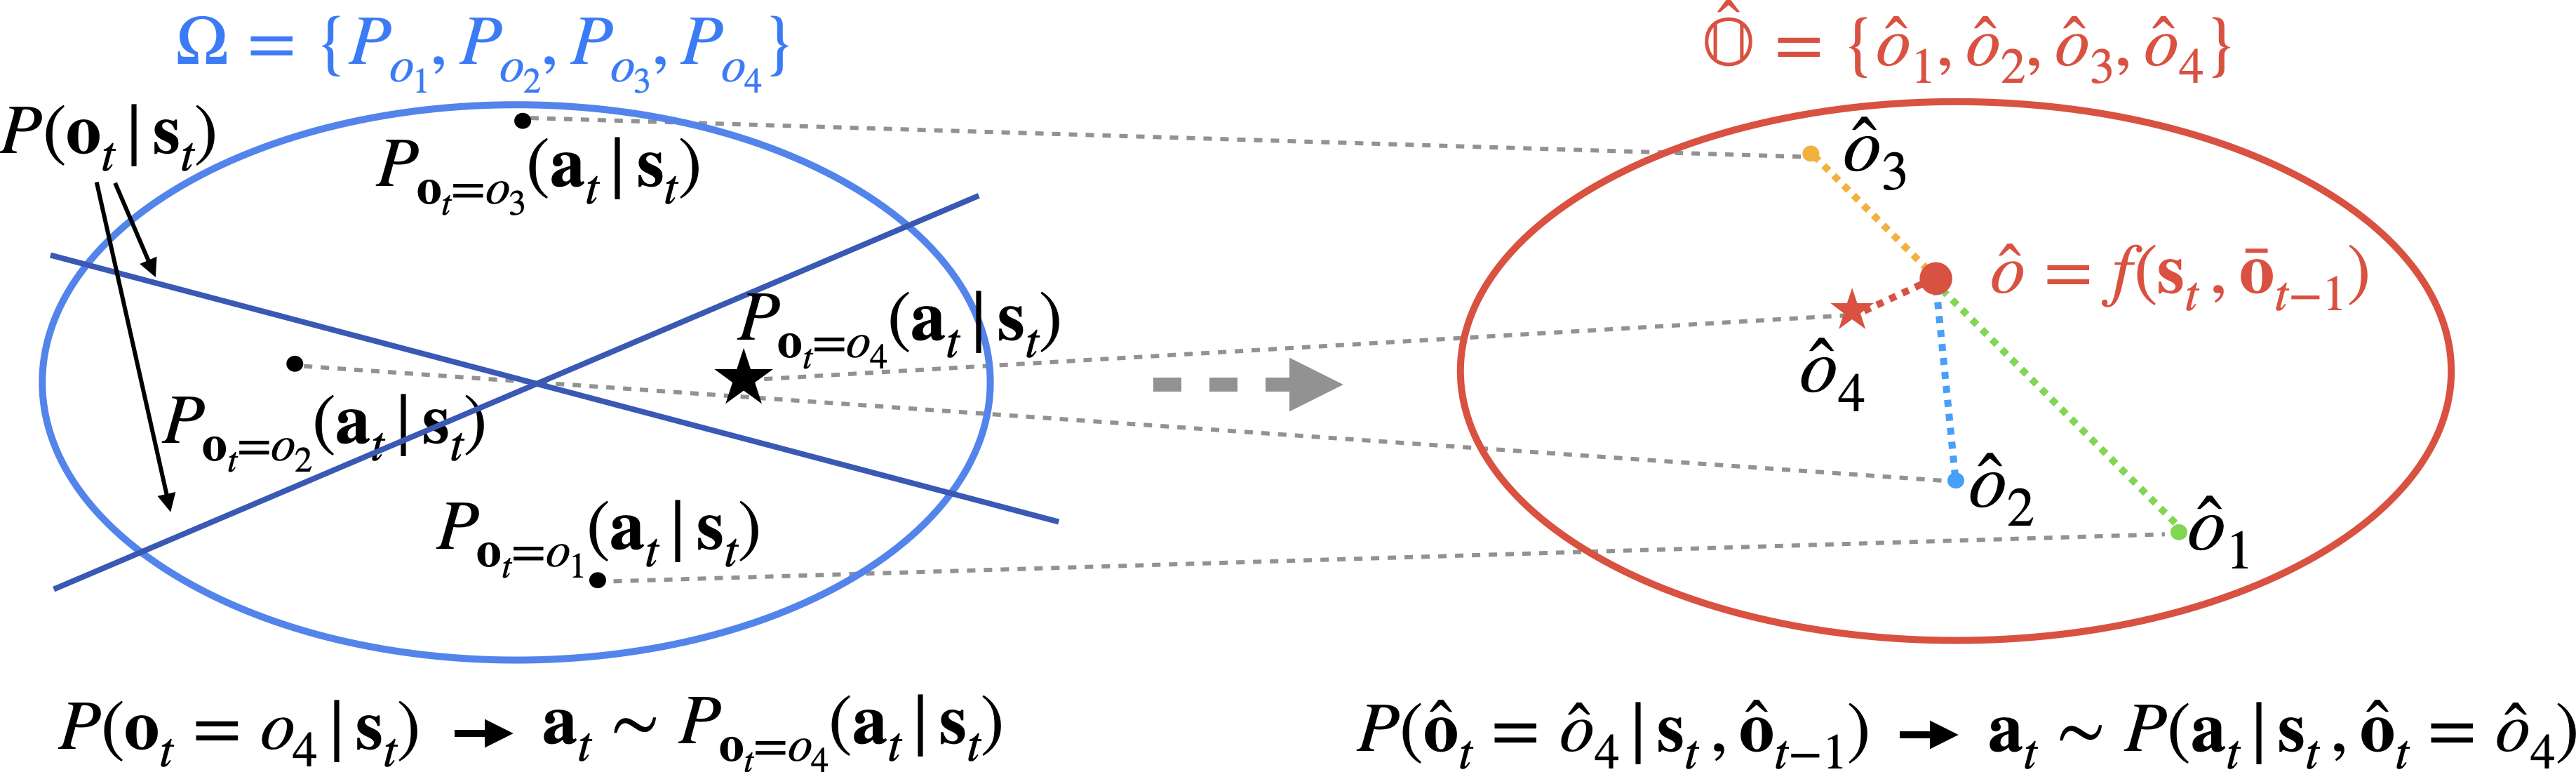
\includegraphics[width=0.9\linewidth]{figures/O2V_Manifold.png}\\
%  \centering
%   \caption{\label{fig:o2v_manifold} Illustrations of
%     \blue{\emph{SMDP-Option} Classification} on \blue{Statistical
%       Manifold} v.s. \red{\emph{MDP-Option} Clustering} on
%     \red{Parametric Space}. On Statistical Manifold, for $M$
%     options there are \blue{$M$ action policies} to learn.
%     Selecting options is analogously \blue{learning
%       classification hyperplanes}. On Parametric Space, for $M$
%     options there are \red{$M$ embedding centroids} to learn yet
%     all embeddings \red{share a single action policy (decoder)}.
%     Selecting options is analogously \red{assigning the closest
%       centroid to the hyperplace $[\rvs_t,\rvo_{t-1}]$}.}
% \end{figure*}

It is worth to point out that, due to space limitation we have to
solely focus on proposing \emph{MDP-Option} and O2V, and
designing experiments to address that O2V achieves at least the
same performance as \emph{SMDP-Option}. Since \emph{MDP-Option}
is equivalent to \emph{SMDP-Option}, it still shares many
identified limitations such as ``the dominant skill problem''
\cite{vezhnevets2017feudal,zhang2019dac} as identified in Section
\ref{sec:exp_ext}. As briefly discussed in Appendix
\ref{sec:append_gist}, \emph{MDP-Option} actually gives rise to
efficient solutions to many identified limitations of
\emph{SMDP-Option} yet have to be deferred to our future works.
Our main contributions are: (1) proposing the \emph{MDP-Option},
a MDP equivalence of \emph{SMDP-Option}, and developing the
bellman equation and gradient theorems; (2) proposing option
embedding vectors, the first distributed representations of
options; (3) proposing the first Attention
\cite{vaswani2017attention} based Encoder-Decoder architecture,
the Option2Vec (O2V) architecture, for learning options with much
better scalability, smaller variance and faster convergence; (4)
demonstrating option embeddings are interpretable, which is a key
property for developing real-world RL applications (e.g. ensuring
safety for human).

% A better way to employ large scale computability. treated as
% undirected graph. learn dependencies end-to-end manner.
% interpretability; safety

% To the best of our knowledge, MDP-Skill is the first MDP enables
% distributed representations of temporal abstractions. O2V is the
% first embedding, attention and encoder-decoder.

% skill embedding can be seen as a minimal (amy zhang iclr2021)
% causal set describing temporal-state (dynamic aware) irrelevant
% by adding extra in objective (feudal net).

% As explained in Appendix \ref{sec:appen_gist}, first-order markov
% formulated MDP-Skill did not fully exploit the potential of O2V. a
% Deep (multi-hierarchy) Wide (higher-order) MDP-Skill will fully
% unleash the power of O2V and gives rise to a general-purpose
% large-scale pre-training framework in RL. We focus this work on
% proposing MDP-Skill and O2V and will explore DWO2V in the future
% work.

% % \item Large variance
% %   \cite{zhang2019dac,haarnoja2018soft}: SMDP
% %   algorithms are notoriously sensitive to hyperparameters . Due
% %   to the SMDP formulation, more stable Markov Decision Process
% %   (MDP) policy gradient algorithms cannot be used.

% % \begin{enumerate}
% % \item O2V is more sample efficient, because a) O2V is MDP
% %   formulated, thus sample at each time step can be used to update
% %   the skill policy; and b) Only one action policy decoder is
% %   needed. It learns to decode each dimension of the skill context
% %   vector at each time step whichever skill is activated;
% % \item O2V has smaller variance, because a) The skill value upon
% %   arrival function (Eq.~(\ref{eq:sa_v})) is theoretically and
% %   empirically proven to have smaller variance than the
% %   conventional value function; and b) O2V only needs to train two
% %   (skill and action) policy networks; and c) O2V can employ more
% %   stable MDP based policy gradient algorithms (e.g.
% %   PPO~\cite{schulman2017proximal});
% % \item O2V has better scalability, because a) Regardless of the
% %   number of skills, only two policies need to be trained; and b)
% %   Adding one more skill is as cheap as adding a context vector;
% %   % to write: disentangle; exploration; convergence speed;
% %   % interpretability; generalization
% % \item O2V is more effective, because a) On infinite-horizon
% %   environments, O2V significantly outperforms the other models;
% %   and b) On transfer learning environments, O2V ranks the first in
% %   5 out of 6 environments and shows its advantages in knowledge
% %   reuse tasks;
% % \item O2V has better interpretability. Unlike the option framework
% %   encodes abstract knowledge implicitly in action policies,
% %   knowledge of a skill is explicitly encoded in each dimension of
% %   the skill context vector.
% % \end{enumerate}


% % % Incomplete Ideas:

% % % 1. 问问题,要解决什么问题,在干什么
% % % 2. 当前sota什么状况,但是有什么问题
% % % 3. 你做了啥,为啥能解决问题
% % % 4. 你这东西有啥特点
% % % 5. 怎么证明这东西work
% % % 6. Implication 是啥

% % % to write: smaller variance
% % % to write: only one critic
% % % to write: deep large scale; imitation; causual relationship
% % % because each run variance so small; not only exploration.

% % % todo: skill not pg/bp; may be dynamic routing/inference/K-means
% % % is enough. should have much simpler design

% % % todo: why option converges slower than action? disentangle paper

% % % todo: supervised train O2V first -> reinf train O2V; Imitation
% % % Learning (dm-control CMU humanoid-v3)

% % % todo: formal def of the turkey: latent variables between
% % % actions and environment. Not observable but truly exists
% % % ; design an experiment to show this problem

% % % potential problem: currently p(o_t|s_t,o_{t-1}) is updated
% % % using Q(o_t,s_t). Should it be Q(o_t,s_t,o_{t-1})? Should
% % % R_{t+1} depends on o_{t-1}?

% % % Yes it should. Reason:

% % % No it should not. Reason: We should not model environment. This
% % % is model free algo. Even though in reality, environment depends
% % % on latent variable $o_{t-1}$ to give R_{t+1}. But we should not
% % % model this relationship in Q value.
% % % Problem: Q used to update p(o'|s',o) does not consider o
% % % Possible solution: instead of include o in Q, create another
% % % ``latent variable environment reward mechanism'' function.
% % % Explicitly model this latent relationship between skill and
% % % environment's reward

% % % A state-previous-skill pair.
% % % Previous research only consider abstract, did not demonstrate
% % % contextual information. Knowing which action has been done can
% % % help predicting whats the next move. Cooking example
% % % Temporal relationships between skills (skill context) has not
% % % been explored before. Seems to encode only one-step temporal
% % % relationship. In order to encode multi time steps relationships,
% % % one can use longer history by turning into higher order markov,
% % % but still markov. our proof still holds. (e.g. adding temporal
% % % masks back to attention, extending the decoder input vector to a
% % % matrix, where rows are time steps, turn it into a k-order markov
% % % process). Remain open for future work.

% % % todo: explain why attention is not the best

% % % idea: In order to have better temporal representation what has
% % % happened before, need a dynamic routing like forward algorithm
% % % to encode all skills have been taken in time series

% % % idea: maximizing reasoning entropy
% % % statistical random variables decreasing bias increasing variance
% % % reasoning variables decreasing bias decreasing variance;
% % % maximizing reasoning entropy

% % % todo: MDP equi minor contribution
% % % todo: Equations addressed stuffed turkey (skill policy, decoder
% % % in nn)
% % % todo: reasons for oc -> sa based on MDP:

% % % minor contribution: MDP
% % % straight forward extend to deeper layer
% % % NLP interface to understand/instruct which dimension encode
% % % what information

\section{Background}
\label{sec:smdp_option}

\textbf{Markov Decision Process:} A Markov Decision Process
\cite{puterman2014markov} $M=\{\sS,\sA,R,P,\gamma\}$ consists of
a state space $\sS$, an action space $\sA$, a state transition
function $P(\rvs_{t+1}|\rvs_t,\rva_t):
\sS\times\sA\rightarrow\sS$, a discount factor $\gamma\in\sR$,
and a reward function
$R(\rvs,\rva)=\E[r|\rvs,\rva]:\sS\times\sA\rightarrow\sR$ which
is the expectation of the reward $r_{t+1}\in\sR$ received from
the environment after executing action $\rva_t$ at state
$\rvs_t$. A policy
$\pi=P(\rva|\rvs):\sA\times\sS\rightarrow[0,1]$ is a probability
distribution defined over actions conditioning on states. A
discounted return is defined as $G_t =
\sum_k^N\gamma^kr_{t+k+1}$, where $\gamma\in (0,1)$ is a
discounting factor. The value function
$V[\rvs_t]=\E_{\tau\sim\pi}[G_t|\rvs_t]$ is the expected return
starting at state $\rvs_t$ and the trajectory
$\tau=\{\rvs_t,\rva_t,r_{t+1},\rvs_{t+1},\dots\}$ follows policy
$\pi$ thereafter. The action-value function is defined as
$Q[\rvs_t,\rva_t]= \E_{\tau\sim\pi}[G_t|\rvs_t,\rva_t]$.

\textbf{Bisimulation Relation:} Given two processes
$M=\{\sS,\sA,R,P,\gamma\}$ with the trajectory $\tau$ and
$\tilde{M}=\{\tilde{\sS},\sA,\tilde{R},\tilde{P},\tilde{\gamma}\}$
with the trajectory $\tilde{\tau}$. Assume both $M$ and
$\tilde{M}$ share the same action space $\sA$. The equivalence
relation between $M$ and $\tilde{M}$ is defined by
\citename{givan2003equivalence}. An equivalence relation
$\tilde{B}:\tilde{\sS}\rightarrow\sS$ is a \emph{Bisimulation
  Relation} if 1) for any state $\rvs$, there exists an
\emph{one-to-one correspondence} equivalent state $\tilde{\rvs}$
that $\rvs/\tilde{B}=\tilde{\rvs}/\tilde{B}$, or denoted as
$\tilde{B}(\tilde{\rvs})=\rvs$, 2) and the following conditions
hold:
\begin{enumerate}
  \label{def:bisimulate}
\item
  $P(\tau/\tilde{B})\equiv
  P(\tilde{\tau}/\tilde{B}),\;\;\;
  \text{and\;}\tilde{B} \text{\;is a \emph{bijection}},$\\
\item
  $V[\tau/\tilde{B}]\equiv
  V[\tilde{\tau}/\tilde{B}]$
\end{enumerate}

In this paper, we follow this definition to prove the equivalence
relationship.

\textbf{The SMDP-based Option Framework}: In \emph{SMDP-Option}
\cite{sutton1999between,bacon2018temporal}, an option is a triple
$(\sI_o, \pi_o, \beta_o)\in \gO$, where $\gO$ denotes the option
set; the subscript $o\in\sO=\{1,2,\dots,K\}$ is a positive
integer index which denotes the $o$th triple where $K$ is the
number of options; $\sI_o$ is an initiation set indicating where
the option can be initiated;
$\pi_o=P_o(\rva|\rvs):\sA\times\sS\rightarrow[0,1]$ is the action
policy of the $o$th option;
$\beta_o=P_o(\rvb=1|\rvs):\sS\rightarrow[0,1]$ where $\rvb\in
{0,1}$ is a \emph{termination function}. For clarity reasons, we
use $P_o(\rvb=1|\rvs)$ instead of $\beta_o$ which is widely used
in previous option literatures (e.g.
\cite{sutton1999between,bacon2017option}).

A \emph{master policy} $\pi(\rvo|\rvs)=P(\rvo|\rvs)$ where
$\rvo\in\sO$ is used to sample which option will be executed.
Note that we use the bold-case $\rvo$ to denote unrealized random
variables and the light-italic-case $o$ to denote a realized
instantiation. Conventionally, the execution of an option employs
the call-and-return model \cite{sutton1999between}: at time step
$t$, an agent either continues the previously executed option
$\rvo_{t-1}=o$ with probability $P_o(\rvb=0|\rvs)$ and sets
$\rvo_t=\rvo_{t-1}=o$, or terminates $o$ with probability
$P_o(\rvb=1|\rvs)$ and samples a new option $\rvo_t$ from the
master policy $P(\rvo_t|\rvs_t)$. Therefore, the dynamics
(stochastic process) of the option framework is written as:
\begin{align}
  \label{eq:oc_pgm_joint}
  P(\tau) = &P(\rvs_0)P(\rvo_0)P_{o_0}(\rva_0|\rvs_0)\prod_{t=1}^\infty P(\rvs_t|\rvs_{t-1},\rva_{t-1})P_{o_t}(\rva_{t}|\rvs_{t})\nonumber\\
            &[P_{o_{t-1}}(\rvb_t=0|\rvs_t)\1_{\rvo_t=o_{t-1}} +P_{o_{t-1}}(\rvb_t=1|\rvs_t)P(\rvo_t|\rvs_t)].
\end{align}
where $\tau=\{\rvs_0,\rvo_0,\rva_0,\rvs_1,\rvo_1,\rva_1,\ldots\}$
denotes the trajectory of the option framework. $\1$ is an
indicator function and is only true when $\rvo_t=o_{t-1}$ (notice
that $o_{t-1}$ is the realization at $\rvo_{t-1}$). Therefore,
under this formulation the option framework is defined as a
Semi-Markov process since the dependency on an activated option
$o$ can cross a variable amount of time \cite{sutton1999between}.
% For the clarity and page limitation, it is enough to only focus
% on the underlying stochastic processes as marginalized versions
% of decision processes in this paper. The complete decision
% process is deferred in Appendix \ref{sec:appen_oc_pgm}.

\section{MDP Equivalences of the SMDP-based Option Framework}
\label{sec:smdp_mdp_sa}
We prove that \emph{MDP-Option} is equivalent to
\emph{SMDP-Option} under the definition of \emph{bisimulation}
\cite{givan2003equivalence}. To derive Bellman equation for
\emph{MDP-Option}, we develop a novel \emph{Markovian skill-value
  function} $\bar{V}[\rvs_t,\rvo_t]$, which is an unbiased
estimation of the conventional value function $V[\rvs_t]$ and the
variance of $\bar{V}[\rvs_t,\rvo_t]$ is up-bounded by
$V[\rvs_t]$. Based on Bellman equation, policy gradient theorems
for \emph{MDP-Option} are then derived. As a result,
\emph{MDP-Option} is a general-purpose MDP which can be combined
with any policy optimization algorithm off-the-shelf.


In this section, we propose \emph{MDP-Option}, a simple yet
effective option-induced MDP and prove its equivalence (as shown
in Figure \ref{fig:sa_logic}) to \emph{SMDP-Option}. For clarity,
in Section \ref{sec:mdp_option} we first prove an intermediate
equivalence \emph{MDP-Mixture} to bridge the equivalence between
\emph{SMDP-Option} and \emph{MDP-Option}. Based on
\emph{MDP-Mixture}, in Section~\ref{sec:sa_PGM} we propose the
\emph{MDP-Option}, a marginalized variation of the \emph{SMDP-Option}. \emph{MDP-Option}
uses the \emph{skill policy} (Eq.~\ref{eq:sa_pgm_joint}), which
is a marginal distribution, to replace the \emph{master policy}
and \emph{termination function}. In order to derive \emph{MDP-Option}'s
Bellman equation, we propose the novel \emph{Markovian
  skill-value function} (Eq.~\ref{eq:sa_v}) and prove that it is
an unbiased estimation of the conventional value function and its
variance is up-bounded by the conventional value function. Policy
gradient theorems for \emph{MDP-Option} are then derived basing on the
Bellman equation. In Section~\ref{sec:net_arch}, we propose O2V,
which is an implementation of the \emph{MDP-Option} by employing the
Embedding and Attention \cite{vaswani2017attention} techniques.
\begin{figure*}[h!]
 \centering
  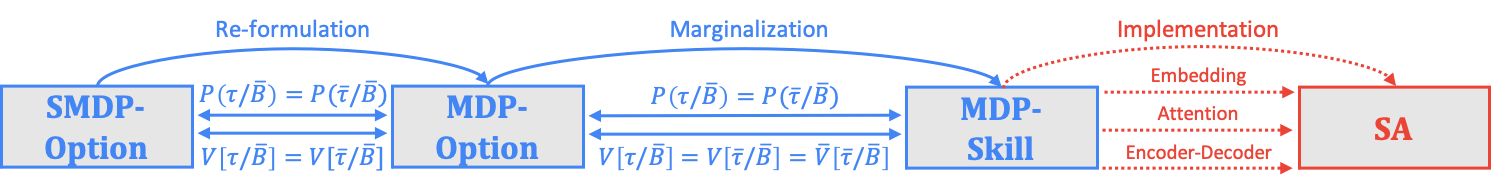
\includegraphics[width=1\linewidth]{figures/SA_Logics.png}\\
  \caption{\label{fig:sa_logic} \red{Bisimulation Relations}.
    \blue{Blue} terms are \blue{Decision Processes}. Solid arrows
    indicate that their equivalences are theoretically justified.
    \red{O2V} is an \red{Architecture} which implements the
    \blue{MDP-Option} by employing Embedding, Attention, and
    Encoder-Decoder techniques. Dashed connections indicate they
    are architecture choices.}
\end{figure*}

% to implement the temporal extension by employing the attention
% mechanism~\cite{vaswani2017attention}. describes the dynamics
% (Markov process) of O2V. Section~\ref{sec:sa_mdp} defines value
% functions on top of the dynamics, thus formulating the MDP.
% Policy gradient theorems are then derived.
% Section~\ref{sec:net_arch} implements O2V by employing neural
% networks and the Multi-Head Attention
% mechanism~\cite{vaswani2017attention}, which enables O2V to
% temporally extend skills in the absence of the termination
% function.


\subsection{The MDP Equivalence (MDP-Mixture) of the Option
  Framework}
\label{sec:mdp_option}
With the definitions of \emph{SMDP-Option} in hand, we now show
how to reformulate it into an MDP-based equivalence
\emph{MDP-Mixture}. The first reformulation is that we follow
\citename{bishop2006pattern}'s formulation of mixture
distributions and redefine the option random variable
$\rvo\in\sO=\{1,2,\dots,K\}$, which was originally defined as an
integer index, but now as a $K$-dimensional one-hot vector
$\bar{\rvo}\in\bar{\sO}=\{0,1\}^K$ where $K$ is the number of
options. The second reformulation is that we exploit the one-hot
vector to reformulate the \emph{termination function} and action
function of each option into two mixture distributions by
introducing extra dependencies on $\bar{\rvo}$:
\begin{align}
  \label{eq:mdp_action_termination}
P(\rva_t|\rvs_t,\bar{\rvo}_t) =
\prod_{o\in\bar{\rvo}_t}P_{o}(\rva_t|\rvs_t)^{o},\nonumber\\
P(\rvb_t|\rvs_t,\bar{\rvo}_{t-1}) =
\prod_{o\in\bar{\rvo}_{t-1}}P_{o}(\rb_t|\rvs_t)^{o},
\end{align}
Since the option random variable $\bar{\rvo}$ is now a one-hot
vector, for $\bar{\rvo}_t=o_t$, by definition only the entry
$o_t=1$ and all the other entry $o\in\sO-\{o_t\}=0$. Therefore,
we have
$P_{o_t}(\rva_t|\rvs_t)=P(\rva_t|\rvs_t,\bar{\rvo}_t=o_t)$ and
$\beta_{o_{t-1}}=P_{o_{t-1}}(\rvb_t=1|\rvs_t)=P(\rvb_t=1|\rvs_t,\bar{\rvo}_{t-1}=o_{t-1})$.

The third reformulation is that we propose a novel \emph{MDP
  mixture master policy}
$P(\bar{\rvo}_t|\rvs_t,\rvb_t,\bar{\rvo}_{t-1})$, which is a
mixture distribution containing the \emph{SMDP master policy} and
a degenerate probability as mixture components by adding two
extra dependencies on $\rvb_t$ and $\bar{\rvo}_{t-1}$:
\begin{equation}
  \label{eq:mdp_oc_po}
P(\bar{\rvo}_t|\rvs_t,\rvb_t,\bar{\rvo}_{t-1}) = P(\bar{\rvo}_t|\rvs_t)^{\rb_t}P(\bar{\rvo}_t|\bar{\rvo}_{t-1})^{1-\rb_t},
\end{equation}
where the indicator function $\1_{\rvo_t=o_{t-1}}$ used in
Eq.\ref{eq:oc_pgm_joint} is now redefined as a degenerate
probability distribution~\cite{puterman2014markov}:
\begin{equation*}
  \label{eq:deg_puterman}
P(\bar{\rvo}_t|\bar{\rvo}_{t-1}) = 
\begin{cases}
  1&\;\text{if } \bar{\rvo}_t=\bar{\rvo}_{t-1},\\
  0&\;\text{if } \bar{\rvo}_t\neq\bar{\rvo}_{t-1}.
\end{cases}
\end{equation*}

We define a function
$\bar{B}(\bar{\rvo})=\bar{\rvo}\cdot\rvd^T:\bar{\sO}\rightarrow\sO$
which maps $\bar{\rvo}$ to $\rvo$, where $\rvd=[1,2,\dots,K]^T$
is a $K$-dimensional constant integer vector and hence
$\bar{B}(\bar{\rvo})=\rvo$. Note that $\bar{B}$ is a
\emph{Bijection} since it is a linear function defined on a
finite integer space. Therefore, by following the definition of
\emph{Bisimulation Relation}, the dynamics of the \emph{SMDP-Option} in
Eq.\ref{eq:oc_pgm_joint} under the Bijection $\bar{B}$ can be
reformulated as:
\begin{align}
  \label{eq:mdp_pgm_joint}
  P(\tau/\bar{B}) =& P(\bar{\tau}/\bar{B})\nonumber\\
                     = &P(\rvs_0)P(\bar{\rvo}_0)P(\rva_0|\rvs_0,\bar{\rvo}_0)\prod_{t=1}^\infty P(\rvs_t|\rvs_{t-1},\rva_{t-1})\nonumber\\
                                            &P(\rva_{t}|\rvs_{t},\bar{\rvo}_{t})\sum_{\rvb_t}P(\rvb_t|\rvs_t,\bar{\rvo}_{t-1})P(\bar{\rvo}_t|\rvb_t,\rvs_t,\bar{\rvo}_{t-1})
\end{align}
where
$\bar{\tau}=\{\rvs_0,\bar{\rvo}_0,\rva_0,\rvs_1,\bar{\rvo}_1,\rva_1,\ldots\}$
is the trajectory of the \emph{MDP-Mixture}.
% Notice that under this formulation, $P(\tau)$ is actually an
% HMM with $\rvs_t$, $\rva_t$ as observable random variables and
% $\rvb_t$, $\bar{\rvo}_t$ as latent variables.

With $P(\tau/\bar{B}) = P(\bar{\tau}/\bar{B})$ in hand, to prove the
equivalence between the \emph{SMDP-Option} and \emph{MDP-Mixture}, we move on to
prove both of them share the same expected reward. This is
non-trivial since compared to the \emph{SMDP-Option}, the MDP
formulation introduces extra dependencies on $\bar{\rvo}$ and
$\rvb$ in Eq.\ref{eq:mdp_pgm_joint} as described above. However,
in Appendix \ref{sec:appen_mdp}, by exploiting conditional
independencies we prove that they do have the same expected
return under the Bijection $\bar{B}$. Therefore, the SMDP-based
option framework has an MDP-based equivalence:
\begin{thm}
  \label{theo:smdp_mdp}
  By the definition of Bisimulation Relation, the SMDP-based
  option framework, which employs Markovian options, has an
  underlying MDP equivalence because:
\end{thm}
\begin{enumerate}
\item
  $P(\tau/\bar{B})
  = P(\bar{\tau}/\bar{B})$
  (Eq. \ref{eq:mdp_pgm_joint}) and $\bar{B}$ is a Bijection.\\
\item
  $V[\tau/\bar{B}]=V[\bar{\tau}/\bar{B}]$
  (Proofs in Appendix \ref{sec:appen_mdp}).
\end{enumerate}

\subsection{Representing Options as Temporal-State Abstraction
  Embeddings}
\label{sec:option_embed}
In this subsection we answer two questions: (1) how to encode
knowledge of $Option^{\textrm{Triple}}$ with option embeddings, \textit{i.e.}, $Option^{\textrm{Embed}}$; and (2) how to achieve
temporal abstractions by replacing the \emph{call-and-return} mode
with a simple \emph{clustering} mechanism. We argue that for
learning temporal abstractions, high-level actions, \textit{i.e.},
$Option^{\textrm{Triple}}$, and the \emph{call-and-return} mode are not
mandatory: temporal abstractions can be achieved by replacing
$Option^{\textrm{Triple}}$ with the a newly defined temporal-state transition-invariant embeddings of hidden variables on which the action policy is conditioned.

We start by reviewing the weaknesses of defining options as high-level actions. Specifically, each $Option^{\textrm{Triple}}$, \textit{i.e.}, a
set of distributions, is analogously a point on a statistical
manifold \cite{amari1987differential}, which is 
computationally expensive to learn. Most literatures ignore
\emph{the initiation} set because of difficulties in learning it
from data \cite{khetarpal2020options}. Learning \emph{master
  policy} is analogously learning classification hyperplanes
\cite{mankowitz2016adaptive} on the statistical manifold. For $M$
hyperplanes, theoretically there are $2^M$ options to be learned as shown in Figure~\ref{fig:o2v_manifold} (left). As pointed out by \citename{bacon2018temporal} (Chapter
3.6), $Option^{\textrm{Triple}}$ cannot at represent knowledge compactly and requires more samples to achieve good performance.
\begin{figure*}[h!]
 \centering
  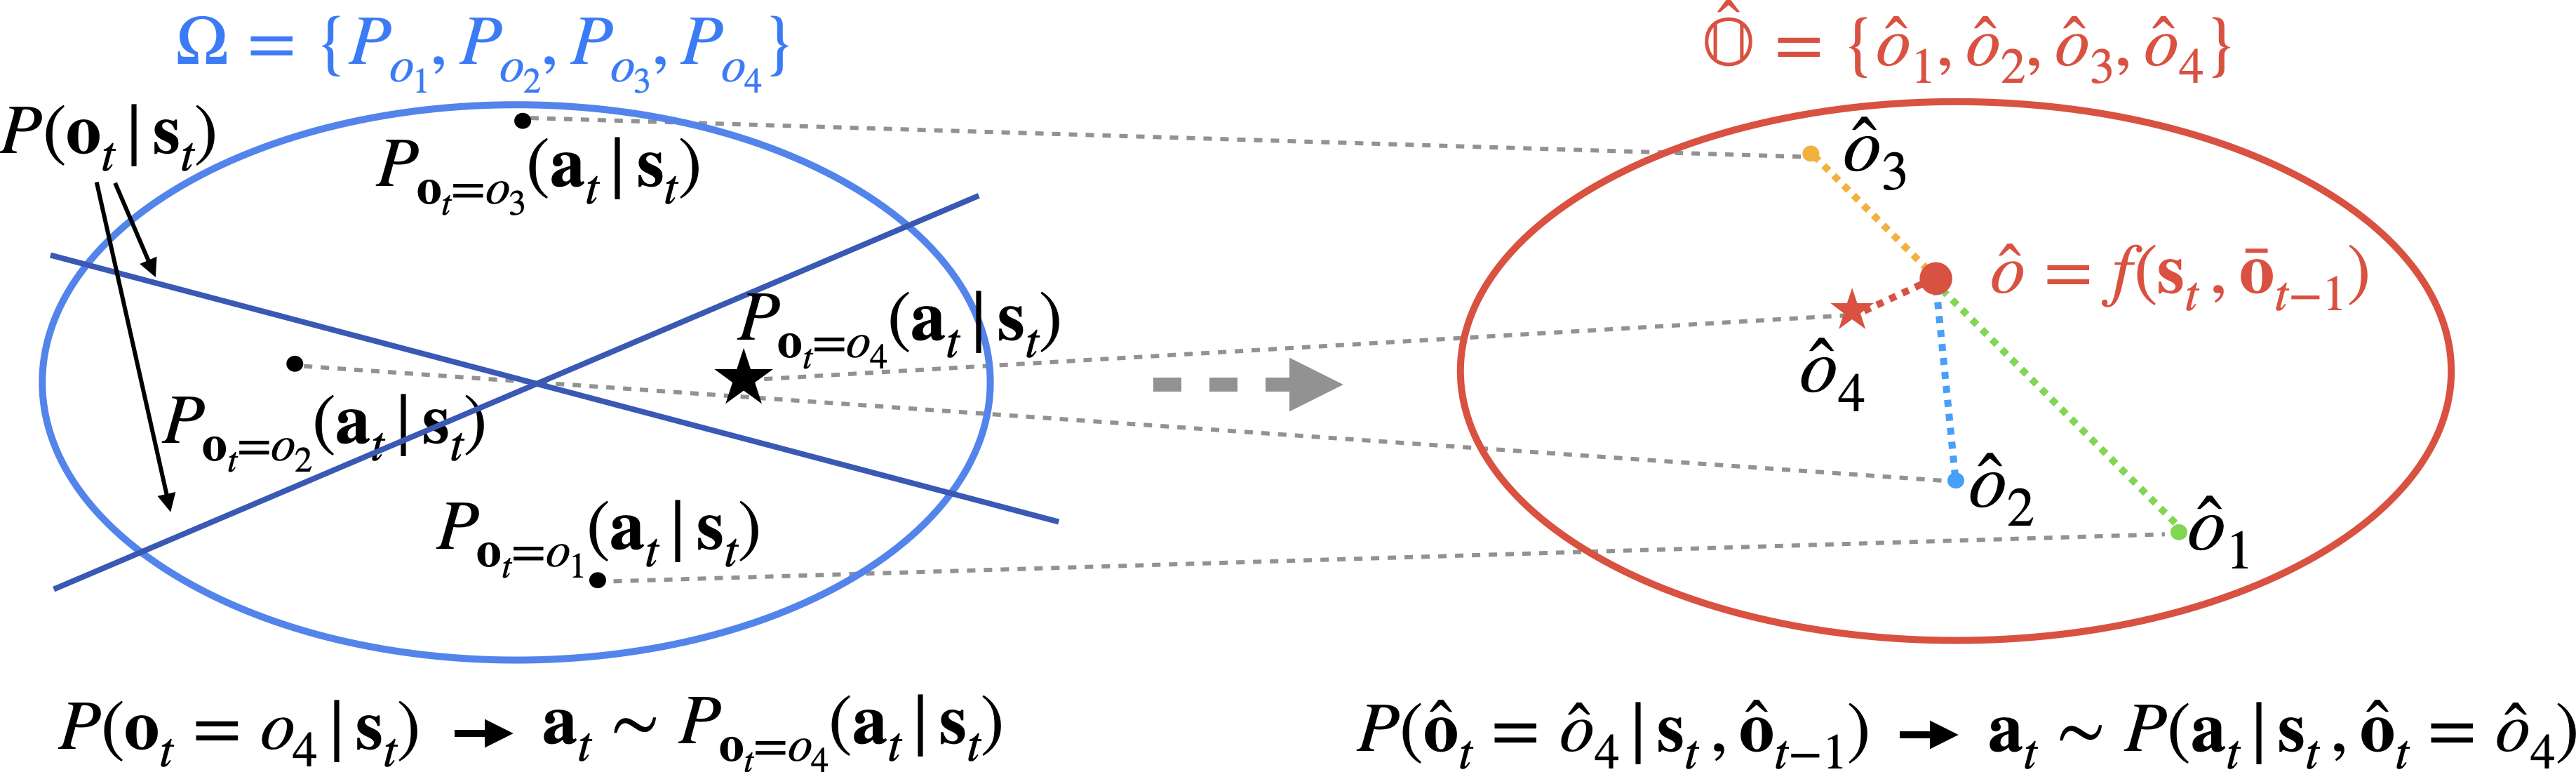
\includegraphics[width=0.9\linewidth]{figures/O2V_Manifold.png}\\
 \centering
  \caption{\label{fig:o2v_manifold} \small
    $Option^{\textrm{Triple}}$ Classification on Statistical
      Manifold (left) v.s. $Option^{\textrm{Embed}}$ Clustering on
    Parametric Space (right). On Statistical Manifold, for $M$
    options there are $M$ intra-option policies to learn
    (for clarity we omit $P_o(\rvb|\rvs)$ and $\sI_o$). Selecting
    options is analogously learning classification 
      hyperplanes (blue lines). On Parametric Space, for $M$
    options there are $M$ embedding centroids to learn yet
    all embeddings share one action policy (decoder).
    Selecting options is analogously assigning the closest
      centroid to the point $[\rvs_t,\rvo_{t-1}]$.}
\end{figure*}

On the other hand, as suggested by
Eq.~(\ref{eq:option_embed_joint}), temporal abstractions can be
achieved more efficiently only by a simple \emph{option
  policy} $P(\bar{\rvo}_t|\rvs_t,\bar{\rvo}_{t-1})$ as long as
there is sufficient context information encoded in $\bar{\rvo}$.
Inspired by word embeddings in
Word2Vec~\cite{mikolov2013distributed}, we address this issue by
representing options as more compact and computationally
efficient embeddings (\textit{i.e.}, semantic space of options).
Specifically, we define a parameter matrix
$\mW_\rvo=[\hat{\rvo}_1,...,\hat{\rvo}_K]\in\sR^{D\times K}$,
where $D$ is the dimension of the vector and $K$ is number of
options. Each real-valued vector $\hat{\rvo}$ is referred to as
an $Option^{\textrm{Embed}}$. As in transformer
\cite{vaswani2017attention}, the option embedding is retrieved
from the embedding matrix by $\hat{\rvo}=\mW_{\rvo}\bar{\rvo}$.
Under this formulation, the hidden variable $\bar{\rvo}$ remains 
the random variable of the \emph{option policy}, while the option 
embedding matrix $\mW_{\rvo}$ is simply the distribution's parameters:
\begin{align}
  \label{eq:option_hat_joint}
  P(\bar{\tau}) =&    
  P(\rvs_0)P(\bar{\rvo}_0)P(\rva_0|\rvs_0,\bar{\rvo}_0)
  \prod_{t=1}^\infty P(\rvs_t|\rvs_{t-1},\rva_{t-1})\nonumber\\
  &P(\rva_{t}|\rvs_{t},\hat{\rvo}_{t})P(\bar{\rvo}_t|\rvs_t,\bar{\rvo}_{t-1};\mW_{\rvo})
\end{align}
where the action policy employs $\mW_{\rvo}$ as a realized hidden
variable rather than parameters, such that
$P(\rva_{t}|\rvs_{t},\hat{\rvo}_{t}=\mW_{\rvo}\bar{\rvo})=P(\rva_{t}|\rvs_{t},\bar{\rvo}_{t},\mW_{\rvo})$.
Note that rather than a mixture of $K$ distributions defined by
Eq.~(\ref{eq:mixture_option_triple}), the action policy is now a
single decoder which is shared by all option embeddings. All
local information of an $Option^{\textrm{Triple}}$ (where to initiate,
what actions to emit and when to terminate) are parameterized as
an embedding vector, \textit{i.e.},
$Option^{\textrm{Embed}}$.

As shown in Figure~\ref{fig:o2v_manifold} (right), $Option^{\textrm{Embed}}$s are
actually clustering centroids on a parametric space, which is
homeomorphic to the statistical manifold. The \emph{option
  policy} maps the observed pair $[\rvs_t,\hat{\rvo}_{t-1}]$ to a
point (detailed implementation is available in Section \ref{sec:net_arch})
on the parametric space. The decision of selecting an option
$\hat{\rvo}_t$ can be made by simply assigning the point to the
closest centroid $\hat{\rvo}^*$, whose distance is estimated
efficiently by employing the Attention mechanism
\cite{vaswani2017attention}. Because a vector is closest to
itself, this mechanism has a natural tendency to continue
$\hat{\rvo}_t=\hat{o}_{t-1}$, yet a significantly different state
$\rvs_t$ will pull the point far enough from $\hat{\rvo}_{t-1}$
and result in another option centroid being assigned. Because the
parametric space is now an ambient space of both state space and
option space, $Option^{\textrm{Embed}}$ combines advantages from both
temporal abstraction and state abstraction
\cite{knoblock1990learning}.

\subsection{Policy Gradient-based Optimization Algorithms}
\label{sec:pgm_opt}

Computing gradients of
Eq.~(\ref{eq:option_hat_joint}) directly is intractable because it
depends on the state transition probability that is unknown under
the model-free RL setting. We address this issue
by first following the RL literature
\cite{sutton2018reinforcement} and define value functions as
expected returns conditioned on the PGM's dynamics. We then
propose a novel \emph{Markovian option-value function} to enable
the derivation of the Bellman equation. We finally derive a
sample efficient policy gradient-based theorems
\cite{sutton2018reinforcement}, which do not involve the state
distribution's gradients, along the expansion of the Bellman
equation. Due to space limitations, we provide the details of all proofs in Appendix~\ref{sec:appen_sa_v_proof}.

Following the RL literature \cite{sutton2018reinforcement}, we
derive the Bellman equation by recursively expanding value
functions. Similar to the value function in Section
\ref{sec:background}, we define the \emph{option-value function}
as the expected return $G_t = \sum_k^N\gamma^kr_{t+k+1}$
conditioned on the current state and option:
\begin{align}
  \label{eq:sa_q_o}
  Q_O[\rvs_t,\bar{\rvo}_{t}]=\E[G_t|\rvs_t,\bar{\rvo}_{t}]
\end{align}
We can further expand the \emph{option-value function} as the
expectation of an \emph{option-action-value function} $Q_A[
\rvs_t,\bar{\rvo}_t,\rva_t]$ by exploiting conditional
independencies encoded in the PGM:
\begin{align}
\label{eq:sa_q_a}
  Q_O[\rvs_t,\bar{\rvo}_{t}]&=\E[G_t|\rvs_t,\bar{\rvo}_{t}]  =\sum_{\rva_t}P(\rva_t|\rvs_t,\bar{\rvo}_{t})\E[G_t|\rvs_t,\bar{\rvo}_t,\rva_t]\nonumber\\
  &=\sum_{\rva_t}P(\rva_t|\rvs_t,\bar{\rvo}_{t})Q_A[ \rvs_t,\bar{\rvo}_t,\rva_t]
\end{align}
In order to establish the connection between the current value
and its successors, \textit{i.e.}, deriving the Bellman equation, we need
to further expand the $Q_A[ \rvs_t,\bar{\rvo}_t,\rva_t]$ to the
next time step:
\begin{align}
  \label{eq:no_recur}
  Q_A[ \rvs_t,\bar{\rvo}_t,\rva_t]&=\E[G_t| \rvs_t,\bar{\rvo}_t,\rva_t]\nonumber\\
  &=
  r(s,a) + \gamma\sum_{\rvs_{t+1}}P(\rvs_{t+1}|\rvs_t,\rva_t)\E[G_t|\rvs_{t+1},\bar{\rvo}_t]
\end{align}
However, as shown in Eq.~(\ref{eq:no_recur}), the last term has an
extra dependency on the hidden variable $\bar{\rvo}_t$. As a
result, the conventional value function $V[\rvs_t]$ does not
yield the recursive formulation required for deriving the Bellman
equation. This issue has not been identified in related
literatures
\cite{henderson2018optiongan,sharma2018directed,shankar2020learning,lee2020learning,zhang2019dac}
which employ the \emph{option policy} as ``one-step option''. In
order to address this issue, we propose a novel \emph{Markovian
  option-value function}
$\bar{V}[\rvs_{t+1},\bar{\rvo}_{t}]=\E[G_t|\rvs_{t+1},\bar{\rvo}_t]$
and prove that:
\begin{prop}
  \label{prop:var_unb}
  $\bar{V}[\rvs_t,\bar{\rvo}_{t-1} ]$ is an unbiased estimation
  of $V[ \rvs_t ]$.
\end{prop}
\begin{prop}
  \label{prop:var_red}
  The variance of $\bar{V}[\rvs_t,\bar{\rvo}_{t-1} ]$ is
  up-bounded by $V[ \rvs_t ]$.
\end{prop}
Proofs are available in Appendix \ref{sec:appen_sa_v_proof}. The
variance-reduction effect is empirically verified in
Section~\ref{sec:exp}. We can then employ the \emph{Markovian
  option-value function} $\bar{V}[\rvs_t,\bar{\rvo}_{t-1}]$ to
derive the Bellman equation:
\begin{equation}
  \label{eq:sa_v}
  \bar{V}[\rvs_{t+1},\bar{\rvo}_{t}]=\E[G_{t+1}|\rvs_{t+1},\bar{\rvo}_{t}]= \sum_{\bar{\rvo}_{t+1}}P(\bar{\rvo}_{t+1}|\rvs_{t+1},\bar{\rvo}_{t})Q_O[ \rvs_{t+1},\bar{\rvo}_{t+1}].
\end{equation}
Expanding $Q_O$ in Eq.~(\ref{eq:sa_v}) through Eq.~(\ref{eq:sa_q_o})
to Eq.~(\ref{eq:no_recur}) gives the recursive formulation of the
Bellman equation. With the Bellman equation in hand, we now are
able to derive policy gradient theorems (Note that to keep notations uncluttered, we use $\theta_{\bar{o}}$ to denote \emph{option policy}'s parameters
$P(\bar{\rvo}_{t}|\rvs,\bar{\rvo}_{t-1};\theta_{\bar{o}})$ and $\theta_a$ to denote action policy's parameters
$P(\rva_t|\rvs_t,\bar{\rvo}_t;\theta_a)$):

\begin{thm}
  \textbf{ Option Policy Gradient Theorem: } Given a stochastic
  \emph{option policy} differentiable in its parameter vector
  $\theta_{\bar{o}}$, the gradient of the expected discounted
  return with respect to $\theta_{\bar{o}}$ is:
  \begin{equation}
    \label{eq:sa_o_grad}
    \frac{\partial \bar{V}[\rvs_t,\bar{\rvo}_{t-1}]}{\partial \theta_{\bar{o}}}=\E[\;\frac{\partial P(\bar{\rvo}'|\rvs',\bar{\rvo})}{\partial \theta_{\bar{o}}}Q_O[\rvs',\bar{\rvo}']\;|\;\rvs_t,\bar{\rvo}_{t-1}],
  \end{equation}
  ~where $\bar{\rvo}'$ is one time step later than $\bar{\rvo}$.
\end{thm}
\begin{thm}
  \textbf{ Action Policy Gradient Theorem: } Given a stochastic action policy
  differentiable in its parameter vector $\theta_a$, the gradient
  of the expected discounted return with respect to $\theta_a$ is:
  \begin{equation}
    \label{eq:sa_a_grad}
      \frac{\partial Q_O[\rvs_t,\bar{\rvo}_t]}{ \partial \theta_a }=\E[\;\frac{\partial P(\rva|\rvs,\bar{\rvo})}{\partial \theta_a}Q_A[ \rvs,\bar{\rvo},\rva]\; | \; \rvs_t,\bar{\rvo}_t].
  \end{equation}
\end{thm}
 Detailed proofs of these two theorems are available
in Appendix~\ref{sec:appen_sa_a_grad}. Similar to
DAC~\cite{zhang2019dac}, our gradient theorems enable a two-stage
optimization scheme (Appendix \ref{sec:append_algo}) for learning
options, in which sample efficient MDP-based algorithms (such as
PPO \cite{witoonchart2017application}) can be employed directly.
It is worth to clarify that the derivation of our theorems is
significantly different from DAC. In DAC, the random variable
$\rvo$ is part of the augmented space $\sS^H$ of the high-level
MDP. On the contrary, we employ an HMM-style PGM and $\bar{\rvo}$
is a hidden variable of the \emph{option policy} and the
\emph{action policy}.

\section{The Option2Vec Architecture (O2V)}
\label{sec:net_arch}
\begin{figure}
  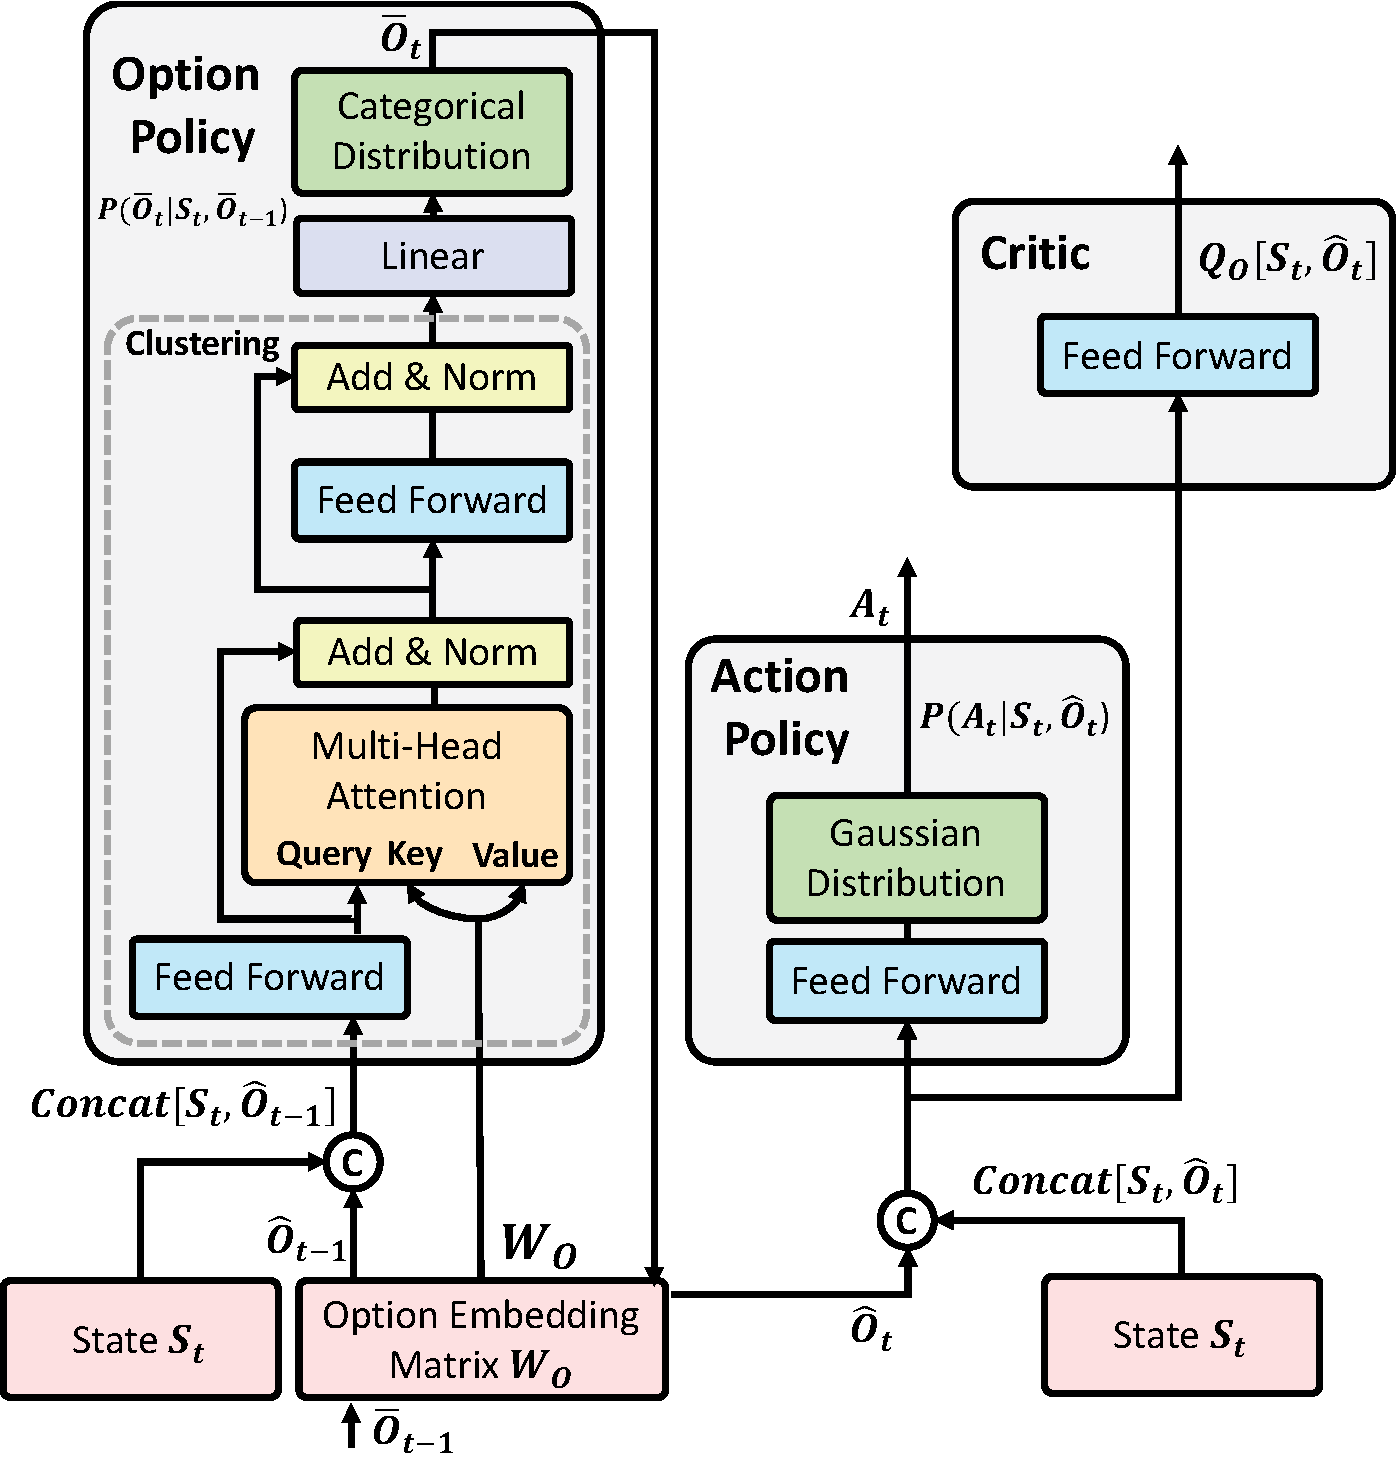
\includegraphics[width=1\linewidth]{./figures/sa_attn_net}
  \caption{\label{fig:sa_net} The Option2Vec Architecture}
\end{figure}

As illustrated in Section~\ref{sec:option_embed}, our main
contributions are representing options as embeddings ($Option^{\textrm{Embed}}$) and
replacing the \emph{call-and-return} mode with the
\emph{clustering mechanism}. Inspired by the \emph{Transformer}
\cite{vaswani2017attention}, in this section we 
implement above mechanisms as Option2Vec, a simple yet
effective Multi-Head Attention (MHA) \cite{vaswani2017attention}
based Encoder-Decoder architecture as shown in Figure~\ref{fig:sa_net}. Due
to space limitations, we explain MHA in
Appendix~\ref{sec:appen_mha}.
In Option2Vec, we implement the \emph{option
  policy} $P(\bar{\rvo}_t|\rvs_t,\bar{\rvo}_{t-1};\mW_{\rvo})$ as
the encoder and treat the option embedding matrix $\mW_{\rvo}$ as
encoder's parameters. Specifically, we define the \emph{option
  encoder} as:
\begin{align}
  \label{eq:net_encoder}
  \bar{\rvo}_t\sim Categorical(Clustering(\rvs_t,\bar{\rvo}_{t-1},\mW_{\rvo}))
\end{align}
where $Categorical(\cdot)$ is a $K$-dimensional categorical distribution, $K$ is the number of options, and distances between the pair $[\rvs_t,\hat{\rvo}_{t-1}]$ (where $\hat{\rvo}_{t-1}=\mW_{\rvo}\bar{\rvo}_{t-1}$) and
all clustering centroids $\hat{\rvo}$ in embedding matrix $\mW_{\rvo}=[\hat{\rvo}_1,...,\hat{\rvo}_K]$ are measured by an
efficient MHA-based \emph{clustering module}:
\begin{align}
  \label{eq:net_encoder}
  &Clustering(\rvs_t,\bar{\rvo}_{t-1},\mW_{\rvo})\nonumber\\
  &=\text{FFN}(\text{MHA}(\text{Query}=\text{FFN}([\rvs_t,\hat{\rvo}_{t-1}]),
\text{Key=Value}=\mW_{\rvo}))
\end{align}
where the concatenated vector $[\rvs_t,\hat{\rvo}_{t-1}=\mW_{\rvo}\bar{\rvo}_{t-1}]$ is
mapped back to a point in the parametric space by employing a
simple Feed-Forward Network. Option2Vec largely improves the
option framework's scalability: under the $Option^{\textrm{Triple}}$
formulation, adding one option means adding two distributions
(normally implemented as neural networks); on the contrary, in
Option2Vec adding one option is as simple as adding one embedding
vector $\hat{\rvo}$. Because the \emph{clustering module} is
MHA-based, the number of parameters for the network stays unchanged
with respect to the number of embeddings in $\mW_{\rvo}$.
With all knowledge of an option (\textit{e.g.}, where to initiate, what
actions to emit, and when to terminate) encoded as an embedding vector $Option^{\textrm{Embed}}$, the
\emph{action policy} can be simply implemented as one decoder,
which learns to decode $\hat{\rvo}_t$ and $\rvs_t$ into primary
actions $\rva_t$.
\begin{align}
  \label{eq:sa_net_action_sample}
  \rva_t \sim Gaussian(\text{FFN}([\rvs_t,\hat{\rvo}_{t}]))
\end{align}
which is shared by all $Option^{\textrm{Embed}}$. This design choice
largely improves Option2Vec's sample efficiency and speed of
convergence: unlike in $Option^{\textrm{Triple}}$ that only the activated
option $\omega_o$'s \emph{intra-option policy} gets updated, the
\emph{action policy} learns to decode $Option^{\textrm{Embed}}$ at every
time step.

Because of the \emph{Markovian option-value function} $\bar{V}[
\rvs_{t+1},\bar{\rvo}_{t} ]$ is an expectation of the
\emph{option-value function} $Q_O[\rvs_{t+1},\bar{\rvo}_{t+1}]$
in Eq.~(\ref{eq:sa_v}), we only need to model only one critic
function: $Q_O=\text{FFN}(\rvs_t,\bar{\rvo}_t)$, where $Q_O$ is
also a decoder of $\rvs_t$ and $\bar{\rvo}_t$. We summarize the
detailed algorithm in Appendix~\ref{sec:append_algo} and upload
our code in supplemental materials.

\section{Experiments}
\label{sec:exp}
% to write: in this section,
In this section, we design experiments to answer five questions:
(Q1) Under the ``one-step option'' setting (Section
\ref{sec:option_pgm}), whether $Option^{\textrm{Embed}}$ is a more compact and effective representation than
$Option^{\textrm{Triple}}$? (Q2) Beyond ``one-step option''
setting, whether Option2Vec can achieve better performance than other option variants and non-option baselines? (Q3) Does $Option^{\textrm{Embed}}$ have a performance boost over other option variants in transfer learning settings? (Q4) Is $Option^{\textrm{Embed}}$ interpretable? (Q5) Whether Option2Vec can temporally extend options under the \emph{clustering} mechanism?

For baselines, we follow DAC~\cite{zhang2019dac}'s open source
implementations and compare our algorithm with six baselines,
five of which are option variants, \textit{i.e.}, DAC+PPO, AHP+PPO
\cite{levy2011unified}, IOPG \cite{smith2018inference}, PPOC
\cite{klissarov2017learnings} and OC \cite{bacon2017option} The
non-option baseline is PPO \cite{schulman2017proximal}. All
baselines' parameters used by DAC remain unchanged other than the
maximum number of training steps: Option2Vec only needs 1 million
steps to converge rather than the 2 million used in DAC. For
single task learning, experiments are conducted on all OpenAI Gym
MuJoCo environments (10 environments) \cite{brockman2016openai}.
For transfer learning, we follow DAC and run 6 pairs of transfer
learning tasks based on DeepMind Control Suite
\cite{tassa2020dmcontrol}. Figures are plotted using DAC's
original script: curves are averaged over 10 independent runs and
smoothed by a sliding window of size 20. Shaded regions indicate
standard deviations. All experiments are run on an Intel® Core™
i9-9900X CPU @ 3.50GHz with a single thread and process. Our
implementation details are summarized in
Appendix~\ref{sec:append_implement}.

For a fair comparison, we follow DAC and use four options in all
implementations. We fix the embedding dimension of
$Option^{\textrm{Embed}}$ to $40$ in all environments, \textit{i.e.},
$\mW_{\rvo}\in \sR^{40\times 4}$. Under this configuration,
Option2Vec only use 15.8\% parameters in all experiments (single
task and transfer learning) compared to the other option
variants. Our code is available in supplemental materials.

\subsection{Single-Task Learning (Q1 \& Q2)}
\label{sec:exp_perf}
To answer Q1, we need to compare the effectiveness of
$Option^{\textrm{Embed}}$ and $Option^{\textrm{Triple}}$ under the same ``one-step
option'' setting. As explained in Section \ref{sec:option_pgm},
although DAC is derived under the ``one-step option'' setting, it still employs \emph{termination
  function} and \emph{master policy} for better performance. Therefore, we
implement a ``DAC-OneStep'' that only employs the \emph{option policy} (code is available in supplemental
materials) and compare its performance with ours in Figure
\ref{fig:ET4}. Experiments show that $Option^{\textrm{Embed}}$
outperforms $Option^{\textrm{Triple}}$ in all environments by a
large margin. This is because, as explained in Section
\ref{sec:option_pgm}, under the ``one-step option'' setting, the
$Option^{\textrm{Triple}}$'s integer \emph{option index} $\rvo$
in Eq.~(\ref{eq:oc_pgm_joint}) contains little context information for the \emph{option policy}
to exploit compared to the $Option^{\textrm{Embed}}$. Moreover,
an $Option^{\textrm{Embed}}$ vector only has $40$ parameters to
train compared to $Option^{\textrm{Triple}}$'s $19$K parameters
(in DAC each \emph{intra-option policy} is a 3-layer FFN). Therefore, $Option^{\textrm{Embed}}$ is a more compact and
effective representation of options compared to
$Option^{\textrm{Triple}}$.
\begin{figure*}[thb]
  \begin{subfigure}{1\textwidth}
    \centering
    
\includegraphics[width=1\linewidth]{figures/ET4.png}
    \caption{\label{fig:ET4}\small Q1: Option2Vec
      v.s. DAC-OneStep}
  \end{subfigure}
  \newline
  \begin{subfigure}{.5\textwidth}
    \centering
    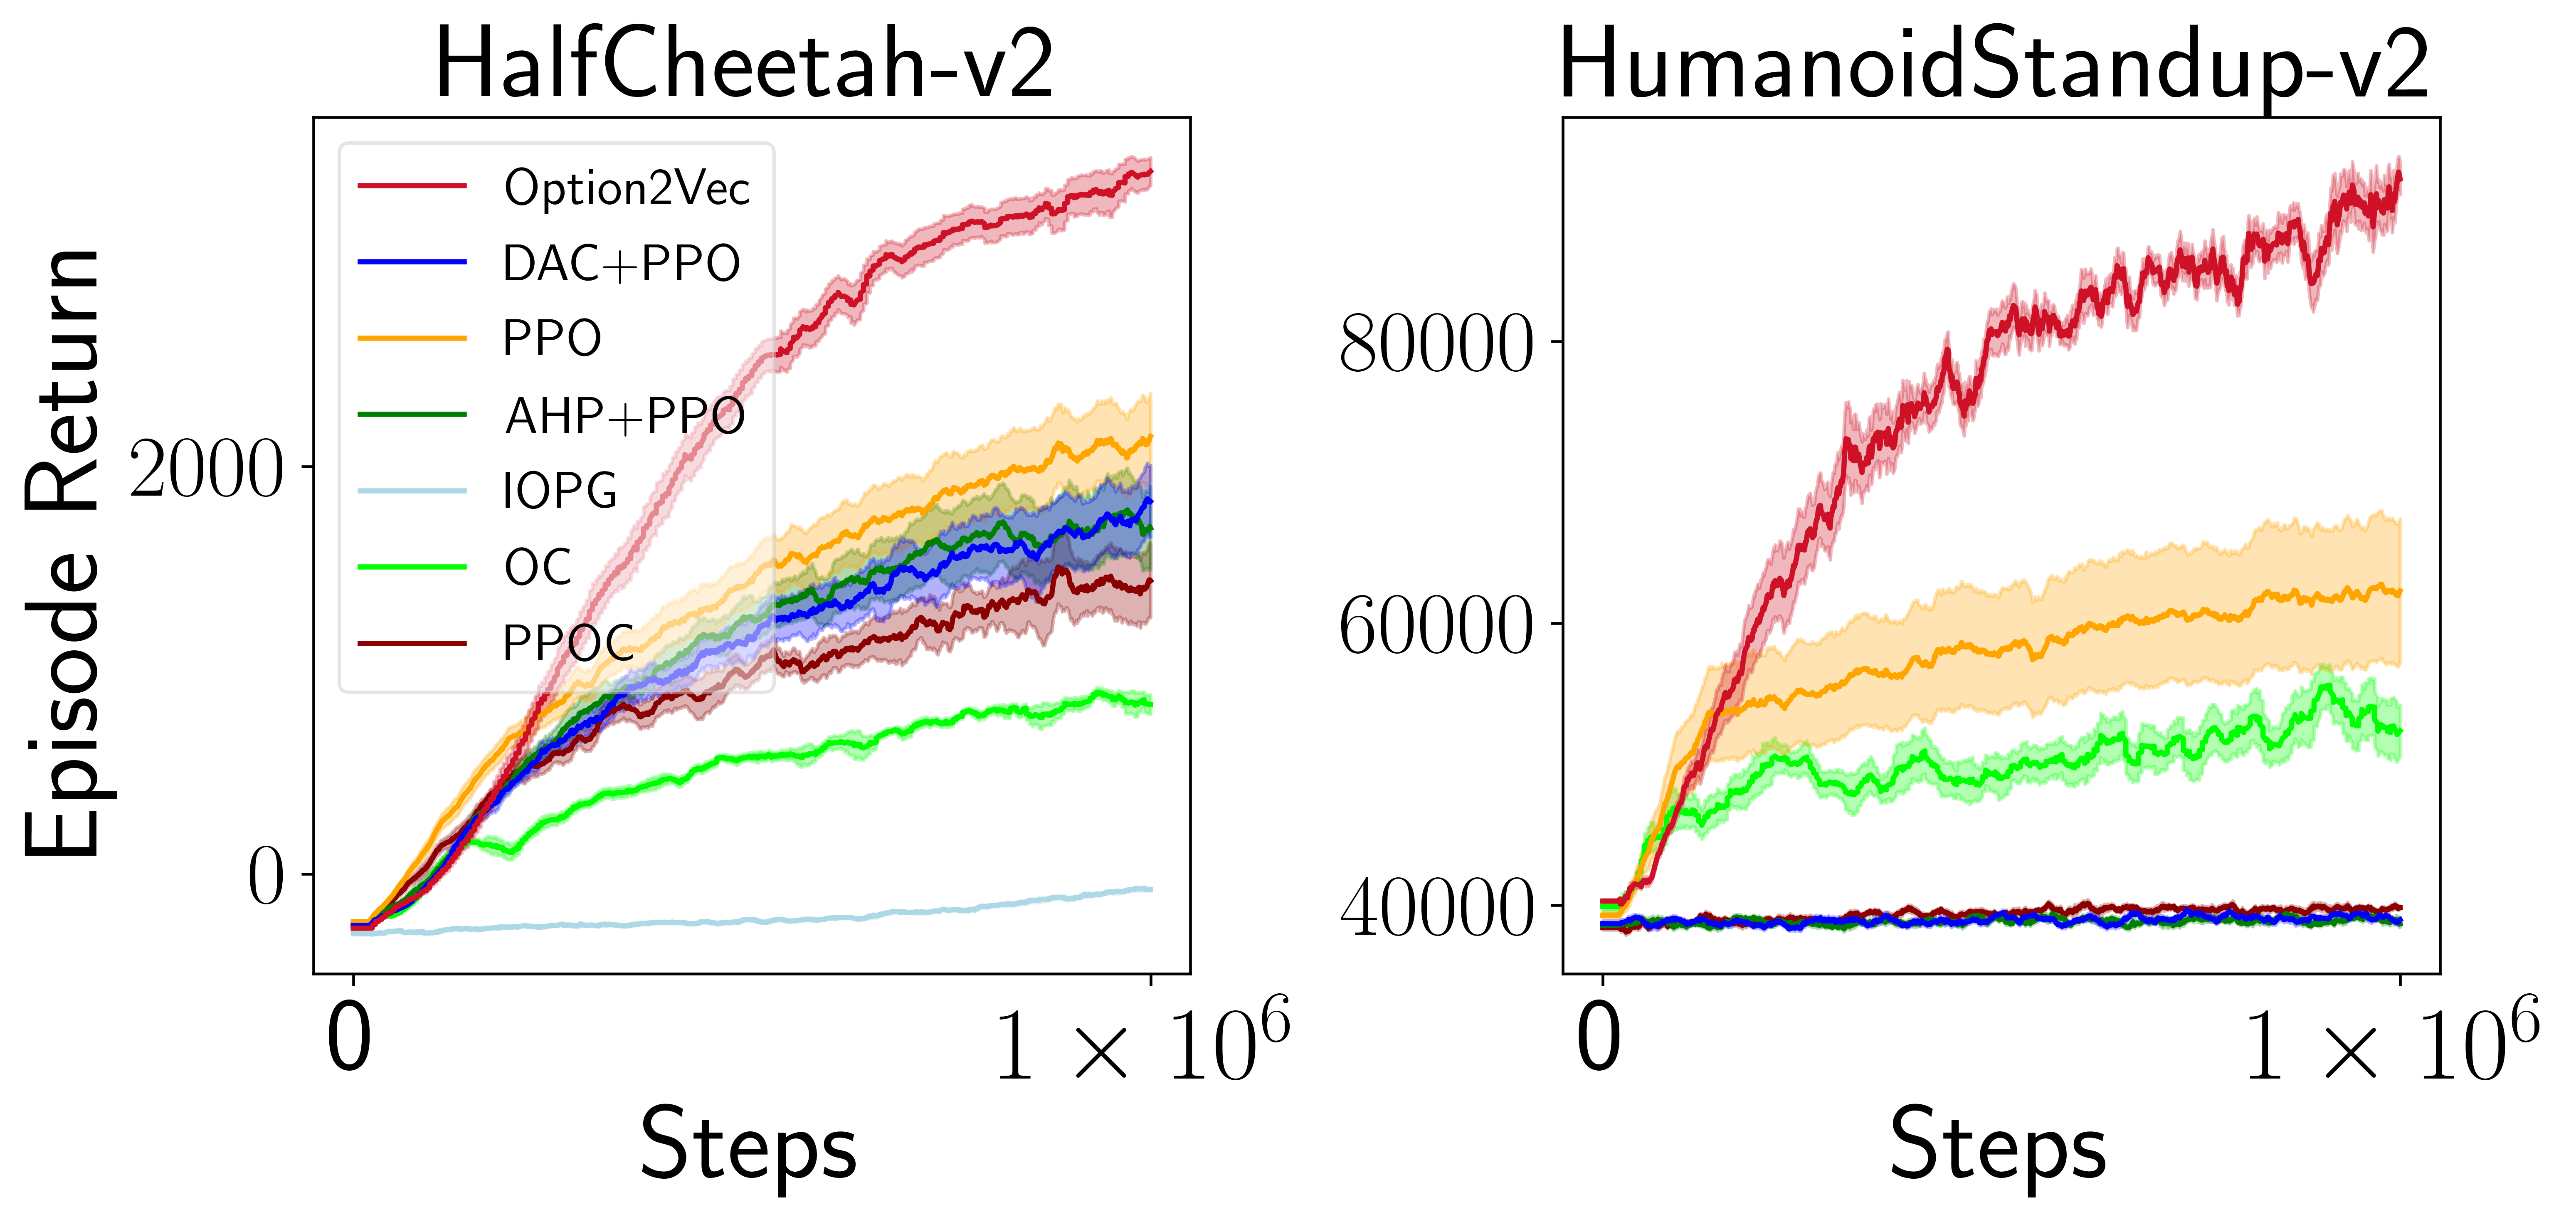
\includegraphics[width=1\linewidth]{figures/Inf2.png}
    \caption{\small Q2: Infinite horizon environments}
    \label{fig:exp_inf}
  \end{subfigure}
  \begin{subfigure}{.5\textwidth}
    \centering
    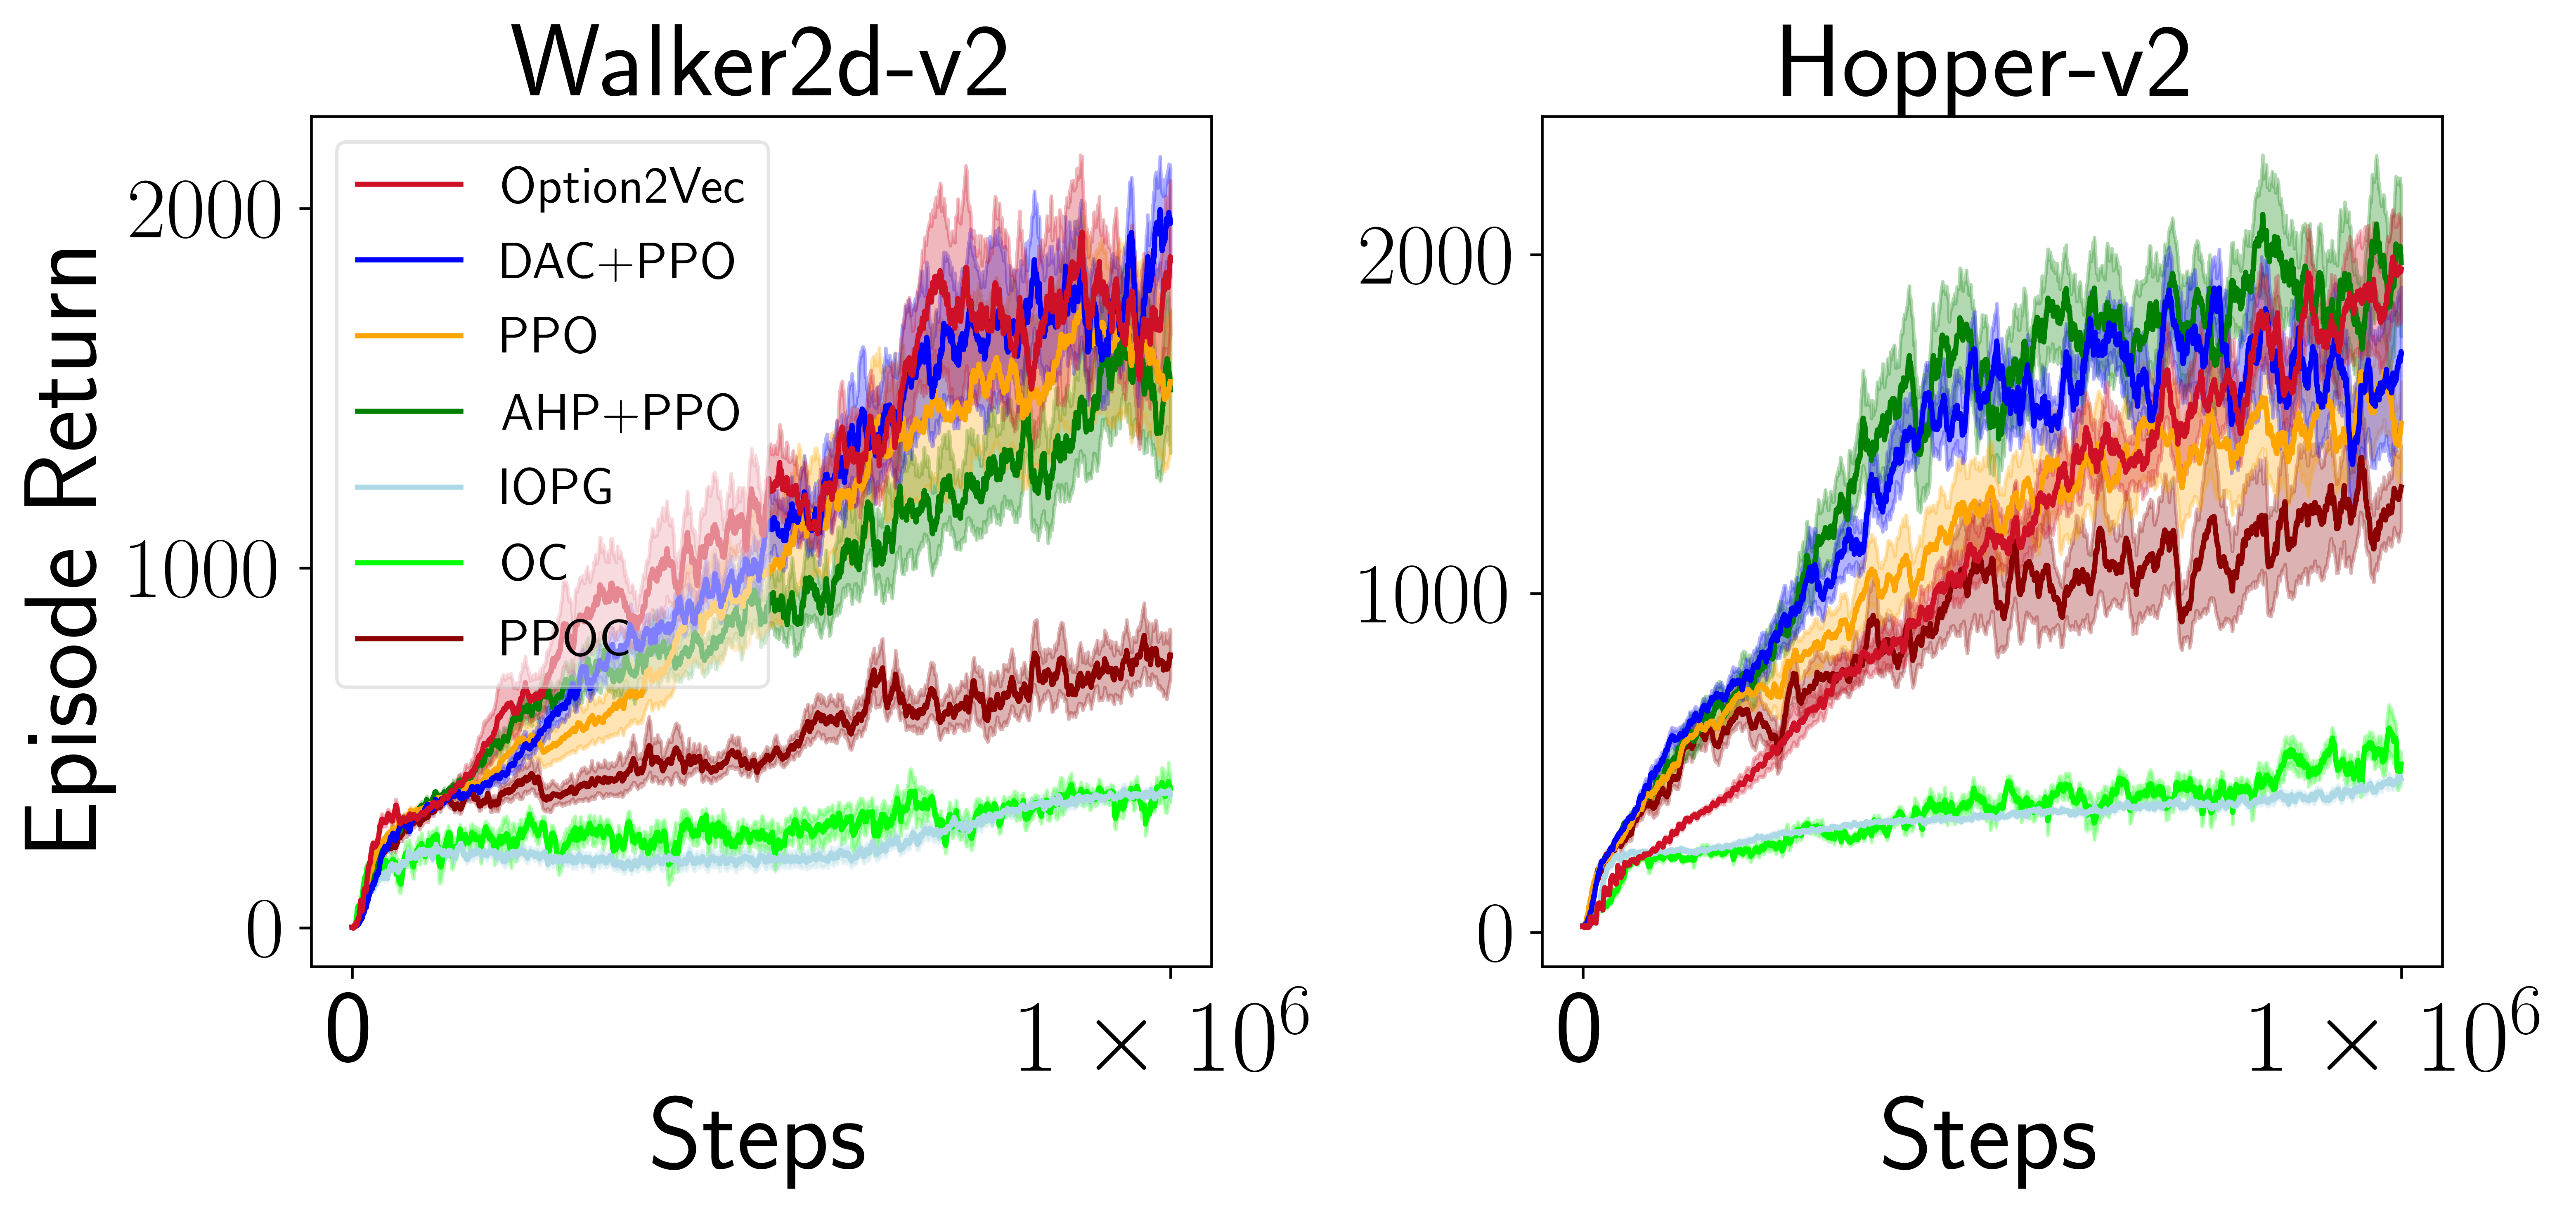
\includegraphics[width=1\linewidth]{figures/F2.png}
    \caption{\small Q2: Finite horizon environments}
    \label{fig:exp_finite}
  \end{subfigure}
  \caption{\small Single-task episodic returns in 4 different environments (\textit{i.e.}, HalfCheetah-v2, HumanoidStandup-v2, Walker2d-v2, and Hopper-v2). Results in all 10 environments are available in Appendix \ref{sec:append_exp_perf}.}
  \label{fig:exp_dac} 
\end{figure*}

To answer Q2, we compare Option2Vec against five different option variants (\textit{i.e.}, DAC+PPO~~\cite{zhang2019dac}, AHP+PPO
\cite{levy2011unified}, IOPG \cite{smith2018inference}, PPOC
\cite{klissarov2017learnings} and OC \cite{bacon2017option}) and PPO~\cite{schulman2017proximal}. It is surprising that Option2Vec shows two different
performance on infinite (Figure \ref{fig:exp_inf}) and and finite
(Figure \ref{fig:exp_finite}) horizon environments. Previous
literatures~\cite{klissarov2017learnings,smith2018inference,harb2018waiting,zhang2019dac}
find that option-based algorithms do not have advantages over
hierarchy-free algorithms on single-task environments. Option2Vec
is also able to achieve comparable performance with state of the arts (Figure
\ref{fig:exp_finite}) but with only 15.8\% parameters.
More importantly, on infinite horizon environments
(Figure~\ref{fig:exp_inf}), Option2Vec's performance
significantly outperforms all baselines with respect to episodic
return, convergence speed, variance between steps, and variance
between 10 runs (Proposition \ref{prop:var_red}). Because
theoretically infinite and finite horizon environments are
identical \cite{sutton2018reinforcement}, we do not have a
theoretical explanation for this performance difference. In
Appendix~\ref{sec:append_gist} we conceptually explain that this
might because conventional value functions are insufficient to
approximate environments in which hidden variables $\rvo$ only
affect rewards but not states. In conclusion, experiment
results show that by employing embeddings and the
\emph{clustering} mechanism (Section \ref{sec:option_embed}),
Option2Vec is at least as effective as other option variants yet
with significantly less computational cost, while has a
significant advantage on infinite horizon.

\subsection{Transfer Learning (Q3)}
\label{sec:transfer}
We run 6 pairs of transfer learning tasks constructed in DAC
based on DeepMind Control Suite \cite{tassa2020dmcontrol}. Each
pair contains two different tasks. To keep consistent with DAC,
we train all models one million steps on the first task and
switch to the second (with $Option^{\textrm{Embed}}$ frozen) to run
another one million steps. Results are reported in
Figure~\ref{fig:transfer}. On the transfer learning (the second)
task, Option2Vec's performance ranks the first in 5 out of 6
environments. This shows Option2Vec's advantages in knowledge
reuse tasks and its performance is at least comparable with other
option variants with significantly less computational cost.

\begin{figure*}[h]
 \centering
  \includegraphics[width=1\linewidth]{./figures/transfer3.png}\\
  \caption{\small\label{fig:transfer} Transfer learning
    results on three pairs of tasks. All 6 pairs of results are available in Appendix.
    \ref{sec:append_exp_perf}}
\end{figure*}

\subsection{Interpretation of Option Embeddings (Q4)}
\label{sec:interpret}
Interpretability is a key property (\textit{e.g.}, ensuring safety to
human, \textit{etc.}) to apply RL agents in
real-world applications. $Option^{\textrm{Embed}}$ has a nature advantage
over $Option^{\textrm{Triple}}$ on interpretability: as word embeddings
\cite{vaswani2017attention}, $Option^{\textrm{Embed}}$ learns a semantic
space of options with each dimension encodes a particular
property and can be interpreted explicitly. As in the capsule
network \cite{sabour2017dynamic}, we first reason each embedding
dimension's semantic by adding perturbations on to it, and
inspecting perturbations' effects on primary actions $\rva$
(Figure \linkblue{6(b)}). Once each dimension is
understood, embeddings become straight forward to interpret by
simply inspecting on which dimensions each embedding $\hat{\rvo}$
(Figure \linkblue{6(a)}) has significant weights, and
interpreting properties of those dimensions
(Figure \linkblue{6(c)} ). Due to space limitations,
more details and GIFs are provided in
Appendix~\ref{sec:append_interpret}.
\begin{center}
\resizebox{1\columnwidth}{!}{%
\begin{tabular}{cc}
  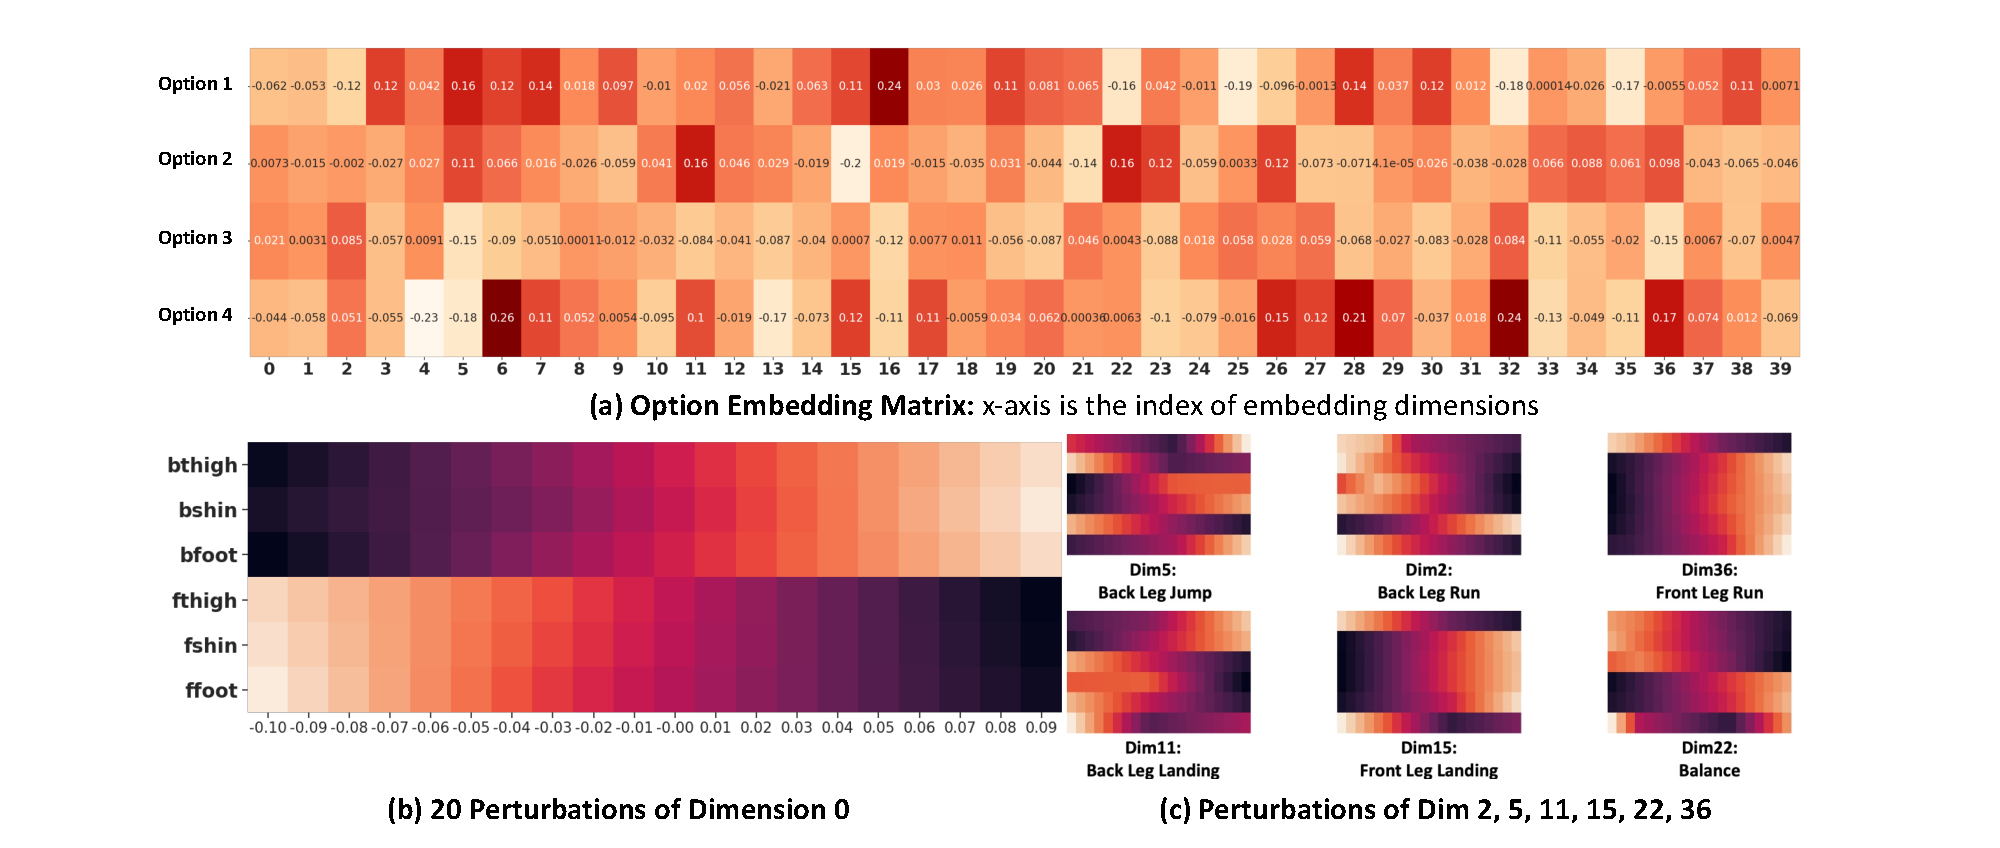
\includegraphics[width=0.7\linewidth]{./figures/interp_joint.pdf}&
                                                                     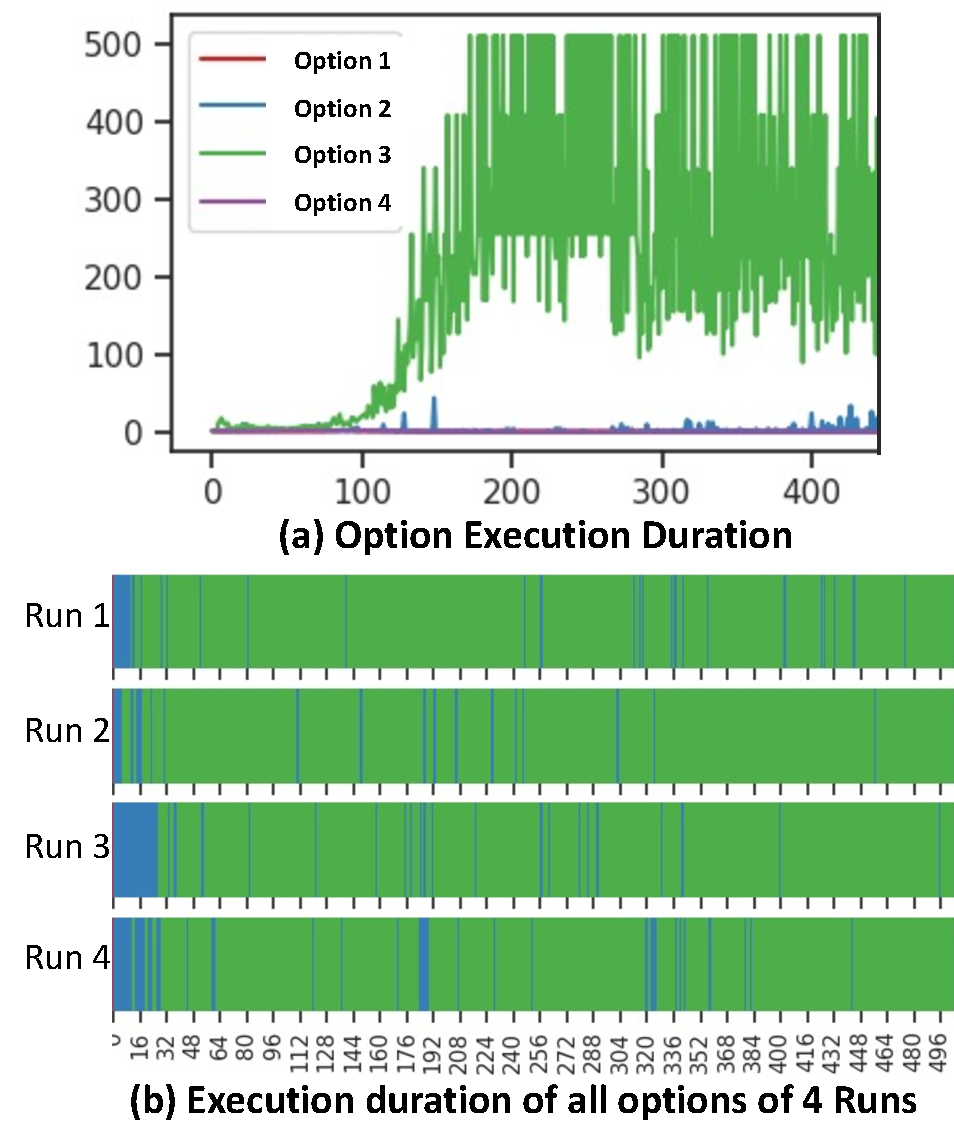
\includegraphics[width=0.275\linewidth]{./figures/duration_main.pdf}\\
  {\small\label{fig:interp_joint}
  Figure 6: Interpretation of option embeddings}&
                                              {\small \label{fig:skill_sequence} Figure 7: Option
                                              Duration Patterns}
\end{tabular}
}
\end{center}

\subsection{Temporal Extension (Q5)}
\label{sec:exp_ext}
We  explained in Section \ref{sec:option_embed} that
\emph{clustering mechanism} is able to temporally extend an
option without the \emph{termination function}. In this subsection we empirically demonstrate this in Figure \linkblue{7}
(more details in Appendix~\ref{sec:append_exp_ext}). 
At the start of training, all options' durations are short, while Option 3's
duration quickly grows. Although this proves that Option2Vec does
temporally extend an option, it also shows that Option2 quickly
dominates the whole episode. The ``dominant skill problem'' is
not unique to Option2Vec, it is a long identified problem of the
option framework \cite{haarnoja2018latent}. However, as shown in
the \linkblue{video}\footnote{\linkblue{https://www.youtube.com/watch?v=F26tcSsIoMA}},
Option2Vec actually learns distinguishable options. Option 3 is a
running forward skill thus it dominates the whole episode. Option
2 is mainly used to recover from falling down thus its duration
decreases with training. In Appendix \ref{sec:append_gist}, we
argue that the dominant skill problem is actually a problem of
learning options at multi-level granularities. Since distances
between embeddings are trivial to measure, $Option^{\textrm{Embed}}$
potentially provides an elegant solution to this problem. We
focus this paper on proposing Option2Vec and will further explore this problem in future works.

\section{Related Works}
\label{sec:review}
% todo: SMDP-style MDP-style
To discover options automatically, \citename{sutton1999between}
proposed Intra-option Q-learning to update the master Q value
function at every time step. However, all policies under this
formulation are approximated implicitly using the Q-learning
method. AHP \cite{levy2011unified} is proposed to unify the
Semi-Markov process into an augmented Markov process and
explicitly learn an ``overall policy'' by applying MDP-based
policy gradient algorithms. However, their method for updating
the master policy is still SMDP-style thus sample inefficient. OC
\cite{bacon2017option} proposes a policy gradient based framework
for explicitly learning intra-option policies and
\emph{termination function}s in an intra-option manner. However,
for the master policy's policy gradients learning, OC still
remains SMDP-style. DAC \cite{zhang2019dac} reformulated the
option framework into two augmented MDPs. Under this formulation, all policies can be modeled explicitly and learned in MDP-style. Policy gradient theorems we derive also follow DAC's efficient
two-stage optimization scheme yet is significantly different
from DAC as explained in Section \ref{sec:pgm_opt}. All above
option variants employ computationally expensive
$Option^{\textrm{Triple}}$ and \emph{call-and-return} mode, while
Option2Vec employs more simple yet efficient
$Option^{\textrm{Embed}}$ and \emph{clustering mechanism}. We
must appreciate that \citename{bacon2018temporal} in his Ph.D.
thesis (Chapter 3.5, 3.6) first conceptually discussed the
possibility of introducing distributed representations into the
option framework. However, to the best of our knowledge,
Option2Vec is the first concrete work that enables learning
options as distributed representations and deriving learning
algorithms.

% With respect to optimization, \citename{zhang2019dac} pointed out
% that a large margin of performance boost of DAC comes from
% Proximal Policy Optimization \cite{schulman2017proximal} (PPO).
% Since Option2Vec is MDP-based, it can be optimized directly with the PPO.
% Recent works show that the option framework trained under
% off-policy \cite{haarnoja2018soft} algorithms outperforms
% on-policy methods. For instance, HO2 \cite{wulfmeier2020data}
% employs a trust-region constrained off-policy algorithm and shows
% that it exhibits significant advantages over on-policy methods on
% both sample efficiency and performance. In this paper, we propose
% Option2Vec as a general HRL framework which can be trained by both
% on-policy and off-policy algorithms. Our main contribution
% focuses on deriving MDPs of Option2Vec and its policy gradient theorems.
% Designing off-policy algorithms for Option2Vec remains open for future
% work.

As for state abstractions, cognitive science experiments
\cite{xia2020temporal} conducted with human participants prove
that human structure, generalize, and adapt past knowledge to new
environments by employing both state abstraction and temporal
abstraction. However, existing RL literature
\cite{hausman2018learning,li2017infogail,tirumala2019exploiting}
only use latent variables to learn state abstractions. Typically,
PEARL \cite{rakelly2019efficient} learns a latent context vector
for each task under the meta-reinforcement learning framework to
improve the agent's sample and transfer learning efficiency.
However, embeddings learned by RL frameworks only encode state
abstraction while Option2Vec is the first option variant learns
abstractions at both state and temporal dimensions.
\section{Conclusions}
\label{sec:conclusion}

In this paper, we proposed a compact and effective embedding representation for the option framework, $Option^{\textrm{Embed}}$.
For learning $Option^{\textrm{Embed}}$, we developed a novel \emph{Markovian Option-Value function} and derived sample efficient policy gradient theorems based on this
value function. We implemented the whole mechanism as Option2Vec, a simple yet effective, transformer-like Attention-based Encoder-Decoder
architecture. Empirical studies showed that $Option^{\textrm{Embed}}$ can significantly outperform $Option^{\textrm{Triple}}$ under the same ``One-step option'' setting in all environments. We also showed that Option2Vec achieves at least comparable performance to other option variants and non-option baselines on finite and transfer learning environments but with only 15.8\% parameters, while has a significant performance boost on infinite environments.
Moreover, option embedding has good interpretability, which is a key property for applying RL agents in real-world applications.

It is also worth mentioning that, the $Option^{\textrm{Embed}}$
establishes a direct connection to causal reinforcement learning
\cite{kolobov2012discovering,perez2020generalized}. If trained
under a model-based setting, $Option^{\textrm{Embed}}$ is a minimal causal
feature set (Theorem 3 \cite{zhang2020learning}) on both temporal
and state dimensions. We will investigate the causal properties of Option2Vec in our future works.


% An example of a floating figure using the graphicx package.
% Note that \label must occur AFTER (or within) \caption.
% For figures, \caption should occur after the \includegraphics.
% Note that IEEEtran v1.7 and later has special internal code that
% is designed to preserve the operation of \label within \caption
% even when the captionsoff option is in effect. However, because
% of issues like this, it may be the safest practice to put all your
% \label just after \caption rather than within \caption{}.
%
% Reminder: the "draftcls" or "draftclsnofoot", not "draft", class
% option should be used if it is desired that the figures are to be
% displayed while in draft mode.
%
%\begin{figure}[!t]
%\centering
%\includegraphics[width=2.5in]{myfigure}
% where an .eps filename suffix will be assumed under latex, 
% and a .pdf suffix will be assumed for pdflatex; or what has been declared
% via \DeclareGraphicsExtensions.
%\caption{Simulation results for the network.}
%\label{fig_sim}
%\end{figure}

% Note that the IEEE typically puts floats only at the top, even when this
% results in a large percentage of a column being occupied by floats.
% However, the Computer Society has been known to put floats at the bottom.


% An example of a double column floating figure using two subfigures.
% (The subfig.sty package must be loaded for this to work.)
% The subfigure \label commands are set within each subfloat command,
% and the \label for the overall figure must come after \caption.
% \hfil is used as a separator to get equal spacing.
% Watch out that the combined width of all the subfigures on a 
% line do not exceed the text width or a line break will occur.
%
%\begin{figure*}[!t]
%\centering
%\subfloat[Case I]{\includegraphics[width=2.5in]{box}%
%\label{fig_first_case}}
%\hfil
%\subfloat[Case II]{\includegraphics[width=2.5in]{box}%
%\label{fig_second_case}}
%\caption{Simulation results for the network.}
%\label{fig_sim}
%\end{figure*}
%
% Note that often IEEE papers with subfigures do not employ subfigure
% captions (using the optional argument to \subfloat[]), but instead will
% reference/describe all of them (a), (b), etc., within the main caption.
% Be aware that for subfig.sty to generate the (a), (b), etc., subfigure
% labels, the optional argument to \subfloat must be present. If a
% subcaption is not desired, just leave its contents blank,
% e.g., \subfloat[].


% An example of a floating table. Note that, for IEEE style tables, the
% \caption command should come BEFORE the table and, given that table
% captions serve much like titles, are usually capitalized except for words
% such as a, an, and, as, at, but, by, for, in, nor, of, on, or, the, to
% and up, which are usually not capitalized unless they are the first or
% last word of the caption. Table text will default to \footnotesize as
% the IEEE normally uses this smaller font for tables.
% The \label must come after \caption as always.
%
%\begin{table}[!t]
%% increase table row spacing, adjust to taste
%\renewcommand{\arraystretch}{1.3}
% if using array.sty, it might be a good idea to tweak the value of
% \extrarowheight as needed to properly center the text within the cells
%\caption{An Example of a Table}
%\label{table_example}
%\centering
%% Some packages, such as MDW tools, offer better commands for making tables
%% than the plain LaTeX2e tabular which is used here.
%\begin{tabular}{|c||c|}
%\hline
%One & Two\\
%\hline
%Three & Four\\
%\hline
%\end{tabular}
%\end{table}


% Note that the IEEE does not put floats in the very first column
% - or typically anywhere on the first page for that matter. Also,
% in-text middle ("here") positioning is typically not used, but it
% is allowed and encouraged for Computer Society conferences (but
% not Computer Society journals). Most IEEE journals/conferences use
% top floats exclusively. 
% Note that, LaTeX2e, unlike IEEE journals/conferences, places
% footnotes above bottom floats. This can be corrected via the
% \fnbelowfloat command of the stfloats package.




\section{Conclusion}
The conclusion goes here.

\subsection{Subsection Heading Here}
Subsection text here.

% needed in second column of first page if using \IEEEpubid
%\IEEEpubidadjcol

\subsubsection{Subsubsection Heading Here}
Subsubsection text here.

% if have a single appendix:
%\appendix[Proof of the Zonklar Equations]
% or
%\appendix  % for no appendix heading
% do not use \section anymore after \appendix, only \section*
% is possibly needed

% use appendices with more than one appendix
% then use \section to start each appendix
% you must declare a \section before using any
% \subsection or using \label (\appendices by itself
% starts a section numbered zero.)
%

\appendices
\section{Proof of the First Zonklar Equation}
Appendix one text goes here.

% you can choose not to have a title for an appendix
% if you want by leaving the argument blank
\section{}
Appendix two text goes here.


% use section* for acknowledgment
\ifCLASSOPTIONcompsoc
  % The Computer Society usually uses the plural form
  \section*{Acknowledgments}
\else
  % regular IEEE prefers the singular form
  \section*{Acknowledgment}
\fi


The authors would like to thank...


% Can use something like this to put references on a page
% by themselves when using endfloat and the captionsoff option.
\ifCLASSOPTIONcaptionsoff
  \newpage
\fi

% trigger a \newpage just before the given reference
% number - used to balance the columns on the last page
% adjust value as needed - may need to be readjusted if
% the document is modified later
%\IEEEtriggeratref{8}
% The "triggered" command can be changed if desired:
%\IEEEtriggercmd{\enlargethispage{-5in}}

% references section

% can use a bibliography generated by BibTeX as a .bbl file
% BibTeX documentation can be easily obtained at:
% http://mirror.ctan.org/biblio/bibtex/contrib/doc/
% The IEEEtran BibTeX style support page is at:
% http://www.michaelshell.org/tex/ieeetran/bibtex/
\bibliography{Bibs/hrl,Bibs/fin,Bibs/lit,Bibs/sa,Bibs/causal,Bibs/IL}
\bibliographystyle{IEEEtran}
% argument is your BibTeX string definitions and bibliography database(s)
%\bibliography{IEEEabrv,../bib/paper}
%
% <OR> manually copy in the resultant .bbl file
% set second argument of \begin to the number of references
% (used to reserve space for the reference number labels box)

% biography section
% 
% If you have an EPS/PDF photo (graphicx package needed) extra braces are
% needed around the contents of the optional argument to biography to prevent
% the LaTeX parser from getting confused when it sees the complicated
% \includegraphics command within an optional argument. (You could create
% your own custom macro containing the \includegraphics command to make things
% simpler here.)
%\begin{IEEEbiography}[{\includegraphics[width=1in,height=1.25in,clip,keepaspectratio]{mshell}}]{Michael Shell}
% or if you just want to reserve a space for a photo:

\begin{IEEEbiography}{Michael Shell}
Biography text here.
\end{IEEEbiography}

% if you will not have a photo at all:
\begin{IEEEbiographynophoto}{John Doe}
Biography text here.
\end{IEEEbiographynophoto}

% insert where needed to balance the two columns on the last page with
% biographies
%\newpage

\begin{IEEEbiographynophoto}{Jane Doe}
Biography text here.
\end{IEEEbiographynophoto}

% You can push biographies down or up by placing
% a \vfill before or after them. The appropriate
% use of \vfill depends on what kind of text is
% on the last page and whether or not the columns
% are being equalized.

%\vfill

% Can be used to pull up biographies so that the bottom of the last one
% is flush with the other column.
%\enlargethispage{-5in}



% that's all folks
\end{document}


